	%%%%%%%%%%%%%%%%%%%%%%%%%%%%%%%%%%%%%%%%%
% Friedrich M. Grabner - 01220997
% Masters Project Report
%%%%%%%%%%%%%%%%%%%%%%%%%%%%%%%%%%%%%%%%%

%----------------------------------------------------------------------------------------
%	PACKAGES AND DOCUMENT CONFIGURATIONS
%----------------------------------------------------------------------------------------
\documentclass[11pt, a4paper]{report}
\usepackage{amsmath, amsthm, amssymb}
\usepackage{graphicx} % Required for the inclusion of images
\usepackage{natbib} % Required to change bibliography style to APA
\usepackage[titletoc]{appendix}
\usepackage{nomencl}
\usepackage{setspace}
\usepackage{geometry} 
\usepackage[hidelinks]{hyperref}
\usepackage{subcaption}
\usepackage{xcolor}
\usepackage{lmodern}
\usepackage{listings}
\usepackage[]{nomencl}
\usepackage{multicol}


\lstset{language=[90]Fortran,
  basicstyle=\ttfamily,
  keywordstyle=\color{red},
  commentstyle=\color{green},
  morecomment=[l]{!\ }% Comment only with space after !
}

\lstset{language=xml,
	tabsize=3,
    %frame=lines,
    %caption=Test,
    %label=code:sample,
    frame=shadowbox,
    rulesepcolor=\color{gray},
    xleftmargin=20pt,
    framexleftmargin=15pt,
    keywordstyle=\color{blue}\bf,
    stringstyle=\color{red},
    numbers=left,
    numberstyle=\tiny,
    numbersep=5pt,
    breaklines=true,
    showstringspaces=false,
    basicstyle=\ttfamily,
    emph={food,name,price},emphstyle={\color{magenta}}}

\geometry{a4paper,total={170mm,257mm},left=20mm,top=20mm}

\linespread{1.5}

\setlength\parindent{10pt} % Removes all indentation from paragraphs
\graphicspath{{./images/}}
\DeclareGraphicsExtensions{.pdf,.PDF,.jpg,.JPG,.bmp,.png,.eps,.EPS}
\makenomenclature
%\usepackage{times} % Uncomment to use the Times New Roman font

%as of 11/04/2013 YMC
\newlength{\MiniPageLeft}
\newlength{\MiniPageRight}
\newlength{\MiniPageSmall}
\newlength{\ThisFigureWidth}
\setlength{\MiniPageLeft}{0.5\textwidth}
\setlength{\MiniPageRight}{\textwidth}
\addtolength{\MiniPageRight}{-\MiniPageLeft}
\newlength{\WidthFull}
\setlength{\WidthFull}{1.0\textwidth}
\newlength{\WidthOneVeryLarge}
\setlength{\WidthOneVeryLarge}{.90\textwidth}
\newlength{\WidthOneLarge}
\setlength{\WidthOneLarge}{.80\textwidth}
\newlength{\WidthOne}
\setlength{\WidthOne}{.70\textwidth}
\newlength{\WidthOneSmall}
\setlength{\WidthOneSmall}{.60\textwidth}
\newlength{\WidthOneVerySmall}
\setlength{\WidthOneVerySmall}{.54\textwidth}
\newlength{\WidthTwo}
\setlength{\WidthTwo}{.49\textwidth}
\newlength{\WidthTwoVeryLarge}
\setlength{\WidthTwoVeryLarge}{.58\textwidth}
\newlength{\WidthTwoSmall}
\setlength{\WidthTwoSmall}{.44\textwidth}
\newlength{\WidthTwoVerySmall}
\setlength{\WidthTwoVerySmall}{.4\textwidth}
\newlength{\WidthThreeLarge}
\setlength{\WidthThreeLarge}{.35\textwidth}
\newlength{\WidthThree}
\setlength{\WidthThree}{.32\textwidth}
\newlength{\WidthThreeSmall}
\setlength{\WidthThreeSmall}{.30\textwidth}
\newlength{\WidthThreeVerySmall}
\setlength{\WidthThreeVerySmall}{.25\textwidth}
\newlength{\WidthFour}
\setlength{\WidthFour}{.24\textwidth}
\newlength{\WidthFourSmall}
\setlength{\WidthFourSmall}{.23\textwidth}
\newlength{\WidthFive}
\setlength{\WidthFive}{.19\textwidth}
\newlength{\WidthSix}
\setlength{\WidthSix}{.15\textwidth}
\newlength{\WidthTest}
\setlength{\WidthTest}{1.2\WidthFour}
\newlength{\WidthSpaceTwo}
\setlength{\WidthSpaceTwo}{.47\textwidth}
\newlength{\WidthSpaceThree}
\setlength{\WidthSpaceThree}{.28\textwidth}
\newlength{\WidthSpaceFour}
\setlength{\WidthSpaceFour}{.22\textwidth}

\newcommand{\ITE}{\begin{itemize}}
\newcommand{\ITED}{\end{itemize}}
\newcommand{\ENU}{\begin{enumerate}}
\newcommand{\ENUD}{\end{enumerate}}
%\newcommand{\etal}{\mbox{\textit{et al.}}}
\newcommand{\etal}{{\it et al\/}.\ }
\newcommand{\etall}{{\it et al\/}.,\ }
\newcommand{\eg}{{\it e.g.}, }
\newcommand{\ie}{{\it i.e.}, }
%\newcommand{\Ans}{$-$ }
\newcommand{\Ans}{$\checkmark$ }
\newcommand{\Q}{\textbf{Q}}
\newcommand{\Com}{$\bullet$ }
\newcommand{\redbullet}{\textcolor[rgb]{1.00,0.00,0.00}{$\bullet$}~}
%\newcommand{\Com}{$\bullet$ \textsf{Comment: }}
%
%Slides
\newcommand{\BegS}{\begin{frame}}
\newcommand{\EndS}{\end{frame}}
\newcommand{\BegB}[1]{\begin{block}{#1}}
\newcommand{\EndB}{\end{block}}
\newcommand{\ppause}{\pause}
%
%Maths symbols
\newcommand{\Ac}{{A}}
\newcommand{\AR}{\mathrm{A_R}}
%\newcommand{\CD}{{C_D}}
\newcommand{\CL}{{C'_L}}
\newcommand{\Cf}{C_f}
\newcommand{\Cfo}{C_{f,0}}
\newcommand{\Ca}{{a_\phi}}
\newcommand{\cp}{c_p}
\newcommand{\Cp}{C_p}
\newcommand{\CRe}{C_M}
\newcommand{\Cs}{C_s}
\newcommand{\degree}{$^\circ$}
\newcommand{\degreee}{{$^\circ$} }
\newcommand{\degreeC}{{$^\circ$C}}
\newcommand{\degreC}{^\circ\mathrm{C}}
\newcommand{\DHy}{D_h}
\newcommand{\dpdx}{\frac{dp}{dx}}
\newcommand{\dpdxs}{\left(\frac{dp}{dx}\right)^*}
\newcommand{\dpdxss}{\left(\frac{dp}{dx}\right)^{**}}
\newcommand{\deltap}{\delta^+}
\newcommand{\Deltap}{\Delta^+}
\newcommand{\Deltatp}{\Delta t^+}
\newcommand{\Deltaxp}{\Delta x^+}
\newcommand{\Deltayp}{\Delta y^+}
\newcommand{\Deltaypmax}{\Delta y^+_{max}}
\newcommand{\Deltaypmin}{\Delta y^+_{min}}
\newcommand{\Deltazp}{\Delta z^+}
\newcommand{\DI}{\mbox{DI}}
%\newcommand{\DR}{\mbox{DR}}
%\newcommand{\DR}{$\mathcal{DR}$}
\newcommand{\DR}{\mathcal{DR}}
\newcommand{\DDR}{\Delta \mathcal{DR}}
\newcommand{\DRmax}{\mathcal{DR}_{max}}
\newcommand{\fx}{f_x}
\newcommand{\fy}{f_y}
\newcommand{\fz}{f_z}
\newcommand{\Ip}{I^+}
\newcommand{\lambdap}{\lambda^+}
\newcommand{\lambdat}{\lambda_2}
\newcommand{\lambdatp}{\lambda_2^+}
\newcommand{\lambdatpz}{\lambda_{2,0}^+}
\newcommand{\lambdax}{\lambda_x}
\newcommand{\lambdaxp}{\lambda_x^+}
\newcommand{\lambdaz}{\lambda_z}
\newcommand{\lambdazp}{\lambda_z^+}
\newcommand{\kappap}{\kappa^+}
\newcommand{\kappax}{\kappa_x}
\newcommand{\kappaxp}{\kappa_x^+}
\newcommand{\kappaxpop}{\kappa_{x,opt}^+}
%\newcommand{\kappax}{\kappa_x}
%\newcommand{\kappaxp}{\kappa_x^+}
%\newcommand{\kappaxpop}{\kappa_{x,opt}^+}
\newcommand{\kappaz}{\kappa_z}
\newcommand{\kappazp}{\kappa_z^+}
\newcommand{\kgs}{kg/s}
\newcommand{\kx}{k_x}
\newcommand{\kz}{k_z}
\newcommand{\mdot}{\dot{m}}
\newcommand{\nus}{\nu_{sgs}}
\newcommand{\nut}{\nu_t}
\newcommand{\omegairmsp}{\omega_{i,rms}^+}
\newcommand{\omegap}{\omega^+}
\newcommand{\omegapop}{\omega_{opt}^+}
\newcommand{\omegapopa}{\omega_{opt,200}^+}
\newcommand{\omegax}{\omega_x}
\newcommand{\Omegax}{\Omega_x}
\newcommand{\omegaxplus}{\left<\omega_x|_+\right>}
\newcommand{\omegaxminus}{\left<\omega_x|_-\right>}
\newcommand{\omegaxpplus}{\omega'_x|_+}
\newcommand{\omegaxpminus}{\omega'_x|_-}
\newcommand{\omegay}{\omega_y}
\newcommand{\Omegay}{\Omega_y}
\newcommand{\omegaz}{\omega_z}
\newcommand{\Omegaz}{\Omega_z}
\newcommand{\omegazero}{\omega_0}
\newcommand{\omegapzero}{\omega^+_0}
\newcommand{\Rc}{r_c}
\newcommand{\ReD}{Re_D}
\newcommand{\ReDo}{Re_{D0}}
\newcommand{\ReDn}{Re_{D1}}
\newcommand{\Reh}{Re_h}
\renewcommand{\Reh}{Re}
\newcommand{\ReH}{Re_H}
\newcommand{\Rem}{{Re_m}}
\newcommand{\Remo}{Re_{m 0}}
\newcommand{\Retau}{Re_\tau}
\newcommand{\Retauo}{Re_{\tau 0}}
\newcommand{\Retauu}{{Re_\tau}}
\newcommand{\RetauD}{{Re_\tau^2}}
\newcommand{\Retheta}{{Re_\theta}}
\newcommand{\rms}{{rms}}
\newcommand{\Sij}{S_{ij}}
\newcommand{\tauij}{\tau_{ij}}
\newcommand{\tauw}{\tau_w}
\newcommand{\tauwo}{\tau_{w_0}}
\newcommand{\tauwno}{\tau_{w_{no}}}
\newcommand{\textinblue}{\textcolor{blue}}
\newcommand{\textingreen}{\textcolor{green}}
\newcommand{\textinred}{\textcolor{red}}
\newcommand{\td}{\xi^*}
%\newcommand{\tNon}{\xi}
\newcommand{\tNon}{t}
\newcommand{\testNon}{{$\xi$}}
%\newcommand{\tNon}{t\Umo/R}
\newcommand{\tp}{t^+}
\newcommand{\tRef}{R/\Umo}
\newcommand{\Tavg}{T_{avg}}
\newcommand{\Tmax}{T_{max}}
\newcommand{\Tmin}{T_{min}}
\newcommand{\Trms}{T_{rms}}
\newcommand{\Tb}{\widetilde{T}_m}
\newcommand{\Te}{T_e}
\newcommand{\Tf}{T_f}
\newcommand{\Tm}{T_m}
\newcommand{\Tp}{T^+}
\newcommand{\Tw}{T_w}
\newcommand{\Uc}{U_c}
\newcommand{\Ucp}{U_c^+}
\newcommand{\Uinfty}{{U_\infty}}
\newcommand{\Uinftysq}{{U_\infty^2}}
\newcommand{\Um}{U_m}
\newcommand{\Umo}{U_{m0}}
\newcommand{\Ump}{U_m^+}
\newcommand{\Up}{U^+}
\newcommand{\DUp}{\Delta \Up}
\newcommand{\dUmdt}{{d\Um}/{dt}}
\newcommand{\umax}{u'_{max}}
\newcommand{\up}{u^+}
\newcommand{\urms}{u_{rms}}
\newcommand{\urmsp}{u_{rms}^+}
\newcommand{\ui}{u_i}
\newcommand{\uj}{u_j}
\newcommand{\uk}{u_k}
\newcommand{\uirms}{u_{i,rms}}
\newcommand{\uirmsp}{u_{i,rms}^+}
%\newcommand{\urms}{u'}
%\newcommand{\urmsp}{u'^+}
%\newcommand{\uirms}{u'_i}
%\newcommand{\uirmsp}{u'^+_i}
\newcommand{\utau}{u_\tau}
\newcommand{\vtau}{u_\tau}
%\newcommand{\utauD}{{u_\tau^2}}
\newcommand{\utausq}{{u_\tau^2}}
\newcommand{\utauno}{u_{\tau_{no}}}
\newcommand{\utauo}{u_{\tau_0}}
\newcommand{\utauosq}{u_{\tau_0}^2}
\newcommand{\uu}{\overline{uu}}
\newcommand{\uv}{-\overline{uv}}
\newcommand{\Vcp}{V_c^+}
\newcommand{\Vcpsq}{V_c^{+2}}
\newcommand{\vf}{\overline{v^2}-f}
%\newcommand{\uv}{\overline{u'v'}}
\newcommand{\vmax}{v'_{max}}
\newcommand{\lref}{L_{ref}}
\newcommand{\uref}{U_{ref}}
\newcommand{\vor}{\omega}
\newcommand{\vorp}{\omega^+}
\newcommand{\vpmax}{v'^+_{max}}
%\newcommand{\vrms}{v'}
\newcommand{\vi}{v_i}
\newcommand{\vj}{v_j}
\newcommand{\vk}{v_k}
\newcommand{\vrms}{v_{rms}}
\newcommand{\vrmsp}{v'^+}
\newcommand{\vv}{\overline{vv}}
\newcommand{\vwall}{v'_w}
\newcommand{\vwallp}{v'^+_w}
\newcommand{\wirms}{\omega_{i,rms}}
\newcommand{\Wm}{W_m}
\newcommand{\Wmp}{W_m^+}
\newcommand{\wmax}{w'_{max}}
%\newcommand{\wrms}{w'}
\newcommand{\wi}{w_i}
\newcommand{\wj}{w_j}
\newcommand{\wk}{w_k}
\newcommand{\wrms}{w_{rms}}
\newcommand{\wrmsp}{w'^+}
\newcommand{\ww}{\overline{ww}}
\newcommand{\w}{\omega'}
\newcommand{\wx}{\omega'_x}
\newcommand{\wxz}{\omega'_{x,0}}
\newcommand{\wxmax}{\omega'_{x, max}}
\newcommand{\wxmin}{\omega'_{x, min}}
\newcommand{\wxwall}{\omega'_{x, wall}}
\newcommand{\wxp}{\omega'^+_x}
\newcommand{\wxpz}{\omega'^+_{x,0}}
\newcommand{\wy}{\omega'_y}
\newcommand{\wymax}{\omega'_{y, max}}
\newcommand{\wypmax}{\omega'^+_{y, max}}
\newcommand{\wyp}{\omega'^+_y}
\newcommand{\wz}{\omega'_z}
\newcommand{\wzwall}{\omega'_{z, wall}}
\newcommand{\xp}{x^+}
\newcommand{\yd}{y_d}
\newcommand{\ydo}{y_d^o}
\newcommand{\ydop}{y_{d,op}}
\newcommand{\ydp}{y_d^+}
\newcommand{\ydpl}{\tilde{y}_d^+}
\newcommand{\ydpo}{{y_d^+}_0}
\newcommand{\ydpop}{y_{d,op}^+}
\newcommand{\ydpno}{{y_d^+}_{no}}
\newcommand{\yh}{y/h}
\newcommand{\yp}{y^+}
\newcommand{\ypmax}{y_{max}^+}
\newcommand{\ypmin}{y_{min}^+}
\newcommand{\ypA}{y^+_A}
\newcommand{\ypo}{y^+_0}
\newcommand{\yv}{y_v}
\newcommand{\zp}{z^+}
%
\newcommand{\kxp}{k_x^+}
\newcommand{\kzp}{k_z^+}
\newcommand{\IT}{{IT}}
\newcommand{\PS}{{PS}}
%Battery
\newcommand{\Li}{{{Li-ion}}}
\newcommand{\DOD}{\mathrm{DOD}}
\newcommand{\dUdT}{\frac{dU}{dT}}
\newcommand{\Ea}{E_{act}}
\newcommand{\kph}{km/h}
\newcommand{\SOC}{\mathrm{SOC}}
\newcommand{\Ti}{T_i}
\newcommand{\Tref}{T_{ref}}
\newcommand{\Umax}{U_{max}}
\newcommand{\Umin}{U_{min}}
\newcommand{\Uoc}{{\bf{U}_{oc}}}
\newcommand{\Vcell}{V_{cell}}
\newcommand{\vcell}{v_{cell}}
\newcommand{\vectoru}{\overrightarrow{u}}
\newcommand{\vectoromega}{\overrightarrow{\omega}}
\newcommand{\cbc}{cbc}
\newcommand{\Hij}{H_{ij}}
\newcommand{\Lii}{L_{ii}}
\newcommand{\Lij}{L_{ij}}
\newcommand{\Mii}{M_{ii}}
\newcommand{\Mij}{M_{ij}}
\newcommand{\Nii}{N_{ii}}
\newcommand{\Nij}{N_{ij}}
\newcommand{\mbc}{\mathbf{mbc}}
\newcommand{\nD}{{n/D}}
\newcommand{\nh}{{n+1/2}}
\newcommand{\nmh}{{n-1/2}}
\newcommand{\np}{{n+1}}
\newcommand{\uip}{{u}_i^{n+1}}
\newcommand{\uio}{{u}_i^n}
\newcommand{\uihat}{\widehat{{u}_i}}
\newcommand{\uno}{{u^n}}
\newcommand{\unp}{{u^{n+1}}}
\newcommand{\ustar}{{u}^{*}}
\newcommand{\udstar}{{u}^{**}}
%\newcommand{\stfirst}{stage I}
\newcommand{\stfirst}{IT stage}
%\newcommand{\stsecond}{stage II}
\newcommand{\stsecond}{WT stage}
%\newcommand{\stthird}{stage III}
\newcommand{\stthird}{ST stage}
%\newcommand{\stfourth}{stage IV}
\newcommand{\stfourth}{PS stage}
\newcommand{\tikzcirc}{\protect\tikz \protect\draw[black] (1ex,1ex) circle (1ex) ; }
\newcommand{\tikzsquare}{\protect\tikz \protect\draw [black] (0.1ex,0.1ex) rectangle (2ex,2ex) ; }

\newcommand{\CA}{\mathbb{C}_A}
\newcommand{\KPe}{K_{Pe}}
\newcommand{\Paw}{P_{aw}}
\newcommand{\Pb}{P_b}
\newcommand{\Pe}{P_e}
\newcommand{\Pl}{P_l}
\newcommand{\Ppl}{P_{pl}}
\newcommand{\Raw}{R_{aw}}
\newcommand{\RP}{R_P}
\newcommand{\VA}{V_A}
\newcommand{\ZPe}{Z_{Pe}}

\newcommand{\JHF}{^{F\&P}}
\newcommand{\FP}{^{FP}}
\newcommand{\NEXT}{\hfill \checkmark}
\newcommand{\END}{\hfill END}

%----------------------------------------------------------------------------------------
%	DOCUMENT INFORMATION
%----------------------------------------------------------------------------------------
\newcommand*{\plogo}{\fbox{$\mathcal{PL}$}}

\newcommand*{\titleGM}{\begingroup % Create the command for including the title page in the document
\hbox{ % Horizontal box
\hspace*{0.1\textwidth} % Whitespace to the left of the title page
\rule{1.5pt}{\textheight} % Vertical line
\hspace*{0.05\textwidth} % Whitespace between the vertical line and title page text
\parbox[b]{0.85\textwidth}{ % Paragraph box which restricts text to less than the width of the page

{\noindent\huge\bfseries 
\includegraphics[width=.75\linewidth,  clip=true, trim = 0cm 0cm 0cm 0cm]{imp_logo}
\\[0.5\baselineskip] MSc Thesis: HPC on the Cloud}
\\[2\baselineskip] % Title
{\Large \textit{Author:}}\\ {Friedrich M. Grabner \\ CID - 01220997 \\}\\
{\Large \textit{Supervisor:}}{\\Dr C. Cantwell}\\% Tagline or further description
{\large } % Author name

\vspace{0.05\textheight}
\begin{center}
\textit{Thesis submitted as part of the requirements\\ for the award of the MSc in Advanced Computational Methods for Aeronautics,\\ Flow Management, and Fluid-Structure Interaction
\\ \vspace{0.25cm}in the}\\
\vspace{0.25cm}	
{Department of Aeronautics, Imperial College London.}
\\
\vspace{0.5cm}	
{September 2017}
\end{center}
\vspace{0.15\textheight} % Whitespace between the title block and the publisher

}}
\endgroup}

\newcommand{\subsubsubsection}[1]{
\vspace{.25cm}
\noindent
\textbf{#1}
\newline
}

\definecolor{mygreen}{HTML}{9BCB99}
\definecolor{myred}{HTML}{FF999A}
\definecolor{myblue}{HTML}{9A99FF}
%----------------------------------------------------------------------------------------
%	TITLE PAGE
%----------------------------------------------------------------------------------------
\begin{document}
\titleGM
\thispagestyle{empty}
\pagenumbering{roman}
% ----------------------------------------------------------------
%	ABSTRACT
% ----------------------------------------------------------------
\begin{center}
{\Large\textsc{Imperial College of Science, Technology and Medicine}}\\ \vspace{.25cm}
Faculty of Engineering\\
Department of Aeronautics\\
\vspace{.5cm}
MSc Advanced Computational Methods for Aeronautics, Flow Management, and Fluid-Structure Interaction\\
\vspace{.5cm}
\textbf{HPC on the Cloud}\\
\vspace{.5cm}
Friedrich M. Grabner\\
\vspace{.5cm}
\hrule
\vspace{.75cm}
{\Large \textit{\textbf{Abstract}}}\\
\end{center}
\vspace{.25cm}


\noindent
Nektar++ is a powerful set of libraries which can be used to simulate a number of physical phenomena. Currently users number in the range of low hundreds. A critical obstacle to wide scale adoption, is in part the complexity of using the software. Indeed there is a steep learning curve to both setup a simulation file and specify computational resources correctly. Limiting ourselves to Nektar++'s incompressible Navier-Stokes solver, a graphical user-interface has been developed. Named TemPSS, the interface is hosted on a Java based web platform. Moreover the entire parameter space, of the incompressible flow solver, has been mapped out using XML schema. Functioning input files for the Nektar++ incompressible flow solver are then generated through an XSLT transform, which the user can then use to run their simulation. Verification of the TemPSS interface has then been performed. Comparison of input files created both manually and through TemPSS for three separate test cases. The outputs from testing proved that TemPSS robustly generates functioning input files for Nektar++.
\newpage
%----------------------------------------------------------------------------------------
%	NOMENCLATURE & ACKNOWLEDGEMENTS
%----------------------------------------------------------------------------------------
\chapter*{Acknowledgements}
A number of people also should receive credit for the success of this project.

Firstly, I must thank Dr Chris Cantwell for having a clear idea of what the outcome of this project should be and guiding me through the many libraries contained within Nektar++ with wit. Additionally I would like to thank Dr Jeremy Cohen for all his technical help and insight. Professor John Darlington also requires praise for his interesting remarks regarding the broader picture of TemPSS and libhpc.

Of course I would also like to thank my various colleagues and friends who have made my time at Imperial College an extremely interesting and memorable experience.

A great contribution is also due to my family who supported me throughout my entire education leading to this point!
\newpage

% ----------------------------------------------------------------
%	TABLE OF CONTENTS
% ----------------------------------------------------------------
\newpage
\tableofcontents
\printnomenclature
% ----------------------------------------------------------------
%	LIST OF TABLES AND FIGURES
% ----------------------------------------------------------------
\newpage
\listoffigures

\listoftables
\newpage
%----------------------------------------------------------------------------------------
%	INTRODUCTION
%----------------------------------------------------------------------------------------
\chapter{Introduction}
\pagenumbering{arabic} 
\nomenclature{IaaS}{Infrastructure as a Service}
Over the past decade rapid progress in computing power has made high-order numerical methods feasible in the simulation of a broad range of engineering problems. In addition the availability of IaaS "cloud-computing" facilities, such as the Amazon EC2\cite{Amazon_2013} and Google Compute Engine\cite{Google2015}, has allowed people outside of large institutions with private clusters to gain access to HPC.

Despite the advancements made many people are still reluctant to utilise codes that implement these new methods, preferring to run commercial software on personal machines. This is in part due to the daunting and complex interfaces of open-source solvers, but also due to the large amounts of additional expertise required to successfully run a simulation.

\begin{figure}[htb!]
 \centering
 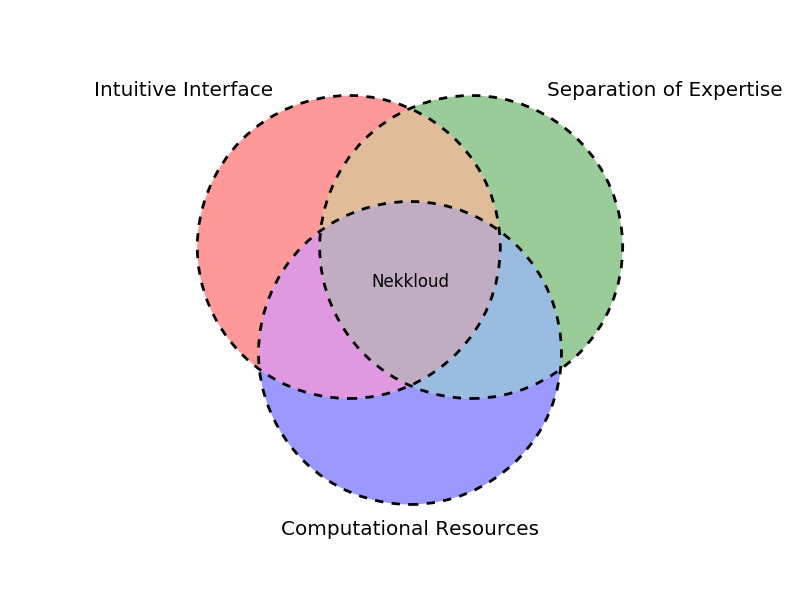
\includegraphics[width=.75\linewidth,  clip=true, trim = .4cm .4cm .4cm .4cm]{venn_diagram}
 \captionof{figure}{Convergence of functionality attempted through Nekkloud.}
 \label{fig:venn_diagram}
\end{figure}

Nektar++\cite{Nektar2015} is an open-source framework of libraries that encapsulate the spectral/hp element method. These libraries can be assembled into a number of different PDE solvers that simulate a variety of physical phenomena. Simulations are defined through the construction of XML\cite{Solo_etal2002} files. Whilst the documentation contains a number of tutorials and other examples, which new users can use to learn more about the code, the XML input files are best developed using a simple text-editor, such as VI or notepad. This requirement immediately alienates those more comfortable with rich text-editors and graphical user interfaces. Furthermore significant knowledge is required to correctly install Nektar++ on all supported platforms. Finally even if correct XMLs have been generated and the software is built correctly, launching a succesful simulation requires definition of computational resources. If Nektar++ is to gain acceptance from the wider community a way of overcoming these issues is needed.

Nekkloud\cite{Cohen_etal2013} is a web-based platform, built on the libhpc framework, through which the Nektar++ solvers can be run. As shown in figure \ref{fig:venn_diagram}, Nekkloud streamlines the use of Nektar++ through opening access to multiple computational resources; separation of expertise into various sections, with the ability to generate many examples; and through providing an intuitive interface encompassing all possible functionality of the solvers but ensuring robust cases are generated.

The project presented within this report aims to develop the latter two of the previous points. Using the TemPSS\cite{Austing_etal2017}, a template and profile manager and editor for the libhpc framework, a graphical interface for Nektar++'s incompressible flow solver has been developed. Through understanding of the constraints present in the code base and numerical methods the interface tries to separate the different domains of expertise required to utilise the code providing a database of example profiles from which new problems can be created.
\newpage

%----------------------------------------------------------------------------------------
%	PROJECT SPECIFICATION
%----------------------------------------------------------------------------------------
\chapter{Project Aims and Objectives}
\label{chap:proj_spec}
\textbf{Project Aims:}
\begin{itemize}
\item Build a web-based graphical user interface, which generates robust and sane input XML files for the incompressible flow solver in Nektar++.
\end{itemize}

The incompressible flow solver was chosen as it has the largest user base and represents a foundation upon which templates for other solvers can be built.
\\ \vspace{.25cm} \\
\textbf{Project Objectives:}
\begin{enumerate}
\item Map and determine the entire parameter space of the incompressible flow solver.
\item Understand and detail the constraints between said simulation parameters.
\item Develop TemPSS transform templates that correctly instantiate all simulation parameters.
\item Represent these parameters and constraints within a logical and intuitive interface.
\item Perform beta testing of the interface with Nektar++ users and implement recommendations.
\item Test the operation of XML generation, through benchmarking against a selection of representative testcases.
\end{enumerate}

%----------------------------------------------------------------------------------------
%	METHOD AND SYSTEMS
%----------------------------------------------------------------------------------------
\newpage
\chapter{Methods and Theory}

\section{Nekkloud, libhpc and TemPSS}
\nomenclature{HPC}{High Performance Computing}
\nomenclature{TemPSS}{Templates and Profiles for Scientific Software}
Nekkloud is the first HPC application to be developed using the libhpc framework. As a web-based platform a number of Nektar++ solvers are available to run on IaaS cloud resources or specific clusters. The libhpc services allows the user to set up compute jobs and select the platforms on which they wish to run.

Sitting beneath libhpc is TemPSS - \textbf{Tem}plates and \textbf{P}rofiles for \textbf{S}cientific \textbf{S}oftware. The TemPSS interface allows the specification of application parameter templates and profiles from which the input XML files for Nektar++ can be generated. As a Java web service, TemPSS is built using Apache Maven and subsequently deployed on an Apache Tomcat server.

\subsection{Design of TemPSS}
The two primary components of the TemPSS interface are the templates and profiles, pictured in figure \ref{fig:TemPSS_interface}.

\subsubsection{Templates}
In order to create an XML input file, using the TemPSS interface, a template must be selected - as shown in the \textcolor{myblue}{blue box} in figure \ref{fig:TemPSS_interface}. Templates define the parameter space avaiable in the tree, see appendix \ref{app:tree_listing}. Moreover the templates available through Nekkloud are each a separate solver package that exist in Nektar++. Though, within the scope of this work, only the incompressible flow solver is considered. Upon selection of a template the relevant tree is loaded into the profile editor as shown highlighted in \textcolor{mygreen}{green box}. 

\begin{figure}[htb!]
 \centering
 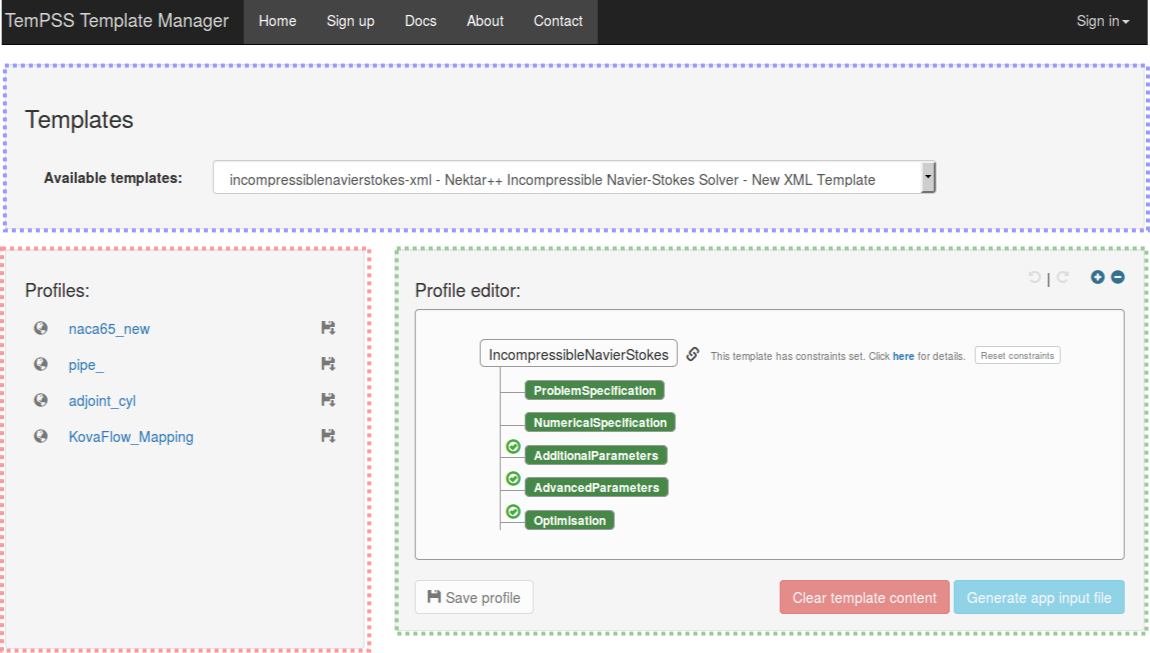
\includegraphics[width=.85\linewidth,  clip=true, trim = 0cm 0cm 0cm 0cm]{TemPSS_interface}
 \captionof{figure}{TemPSS Interface incompressible Navier-Stokes solver template seclected.}
 \label{fig:TemPSS_interface}
\end{figure}

\subsubsection{Profiles}
Profiles are instantiations of templates. A profile contains the values for the entire or part of the template tree. Profiles can then be saved, as seen in the profile box highlighted in \textcolor{myred}{red}. Once a profile is entirely filled then it is possible to transform the template and generate an output XML file.

Profiles can also be saved and shared with other users, this is part of the wider eco-system that Nekkloud is trying to foster. Users who lack expertise in one aspect of the simulation setup are able to look what other users have specified for similar problems. Figure \ref{fig:TemPSS_interface} shows a number of saved profiles available for a user to load and tailor to their requirements.

\subsection{Input to Output}
Built using the Java web service environment, TemPSS uses a number of Java libraries and files to manage the user and profiles database. Additionally these also to define the overall function and look of the interface. 

Structure of template trees, such as that for the incompressible Navier-Stokes solver, are defined by XML schema. These schema are constituted, in part, by further smaller XML style sheets. The final Nektar++ compatible XML is then generated through an XSLT transform.

\subsubsection{XML Structure}
\nomenclature{XML}{Extensible Markup Language}
XML is the chosen text format for both the input file for Nektar++ and schema definition for the TemPSS parameter tree. XML files are structured into multiple hierarchies of parent and child nodes. Figure \ref{fig:XML} shows an example XML schema definition of a forcing function in Nektar++. The parent node is named \texttt{Force}, and it has three children: \texttt{Absorption}, \texttt{Body} and, \texttt{Noise}. The children may also have children, such as \texttt{Absorption} has \texttt{Coeff}, \texttt{RefFlow} and, \texttt{RefFlowTime}. This can go on \textit{ad infinitum}.

\begin{figure}[htb!]
 \centering
 \lstinputlisting{./data/simple.xml}
 \captionof{figure}{Example Xml Schema Defining Part of a TemPSS Tree.}
 \label{fig:XML}
\end{figure}

To define the functionality of a node keywords with additional information can be include in the node head. The options available, to both the parent and child nodes, are given by the standard XSLT library and additional custom options are defined across a number of XML style sheets. 

In figure \ref{fig:XML} the parent node \texttt{Force} uses keywords \texttt{repeatable}, \texttt{paramType}, and \texttt{optional}. Keywords \texttt{repeatable} and \texttt{optional} are defined in the XSL file \texttt{XsdToHtmlTransform.xsl}. These options give the ability to define between $0$ to $\infty$ instances of \texttt{Force}. For example one may wish to have both an absorption and body force, thus the option \texttt{repeatable} allows the addition of instances of this function. In figure \ref{fig:force_tree} we see the manifestation of the \texttt{repeatable} keyword in the form of a plus sign, clicking on this adds an extra instance to the tree. Similarly the \texttt{optional} command is seen in figure \ref{fig:force_tree} as the slider. The slider is coloured green for force, as it has been selected, but red for the other options which are not. This switch allows options to be added in or out of the output easily.

\begin{figure}[htb!]
 \centering
 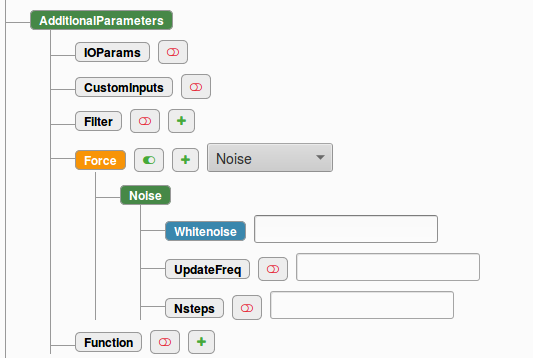
\includegraphics[width=.75\linewidth,  clip=true, trim = 0cm 0cm 0cm 0cm]{force_tree}
 \captionof{figure}{Snippet of Overall Tree Showing Definition of Forcing Function.}
 \label{fig:force_tree}
\end{figure}

The child node \texttt{Noise} is selected in figure \ref{fig:force_tree}. Observing that in the XML structure, figure \ref{fig:XML}, that defines this tree the child of \texttt{Noise} has the nodes \texttt{Whitenoise}, \texttt{UpdateFreq} and \texttt{Nsteps}. These have type defined as positiveDouble - a custom type. Figure \ref{fig:custom_type} shows how using the XSLT standard parameters a new custom type is created which only allows positive doubles to be entered as inputs.

\begin{figure}[htb!]
 \centering
 \lstinputlisting{./data/type.xml}
 \captionof{figure}{Example Custom Node Type Limiting Input to Positive Values.}
 \label{fig:custom_type}
\end{figure}

\subsubsection{XSLT Transform}
\nomenclature{XSLT}{Extensible Stylesheet Language Transformations}
XSLT transforms generated an output XML, compatible with Nektar++, from the instatiated XML schema. XSLT reads the relationships between nodes as a set of paths. Named XPATH, this allows information entered at any node within the TemPSS tree top be accessed and then applied to the output XML. For example in figure \ref{fig:XML} the XPATH to the value of \texttt{UpdateFreq} would be \texttt{Force/Noise/UpdateFreq}.

\begin{figure}[htb!]
 \centering
 \lstinputlisting{./data/transform_parent.xml}
 \captionof{figure}{Example XSLT Transform File	Showing How XSLT Searching for Activated Nodes.}
 \label{fig:xsl_parent}
\end{figure}

In figure \ref{fig:xsl_final} the XPATH of the primary node is seen on line 2. The function \texttt{match} finds the paths specified, in this case \texttt{IncompressibleNavierStokes}, and subsequently writes the XML nodes \texttt{<NEKTAR>} to lines 3 and 8 of the output XML, figure \ref{fig:xml_output}. In order to further instantiate the output XML another template is applied on line 4 of figure \ref{fig:xsl_final}. Here function \texttt{<xsl:apply-templates>} then scans for the path \texttt{AdditionalParametersForce}. If this path exists the template named \texttt{AddForces}, figure \ref{fig:xsl_parent}, is applied.

In the template \texttt{AddForces} the same process is repeated. If the XPATH finds \texttt{Force} in the TemPSS tree the nodes \texttt{<FORCE>} are added, which manifest in the output \ref{fig:xml_output} on lines 3 and 7. As there are a number of options this template performs a number of \texttt{<xsl:if>} tests to check which additional templates should be utilised. Absorption has been selected in the TemPSS tree, thus the \texttt{<xsl:attribute>} places the tag \texttt{TYPE="Absorption"} in the output force node, see line 3 of figure \ref{fig:xml_output}. When the simulation is then run the Nektar++ solver will read this tag and apply an absorption force as desired.

\begin{figure}[htb!]
 \centering
 \lstinputlisting{./data/transform_child.xml}
 \captionof{figure}{Example XSLT transform File Showing XSLT Searching for Values of Nodes.}
 \label{fig:xsl_child}
\end{figure}

\begin{figure}[htb!]
 \centering
 \lstinputlisting{./data/transform_final.xml}
 \captionof{figure}{Example XSLT transform determining overall XML structure.}
 \label{fig:xsl_final}
\end{figure}

Having applied the absorption force tag another template is called, seen in figure \ref{fig:xsl_child}, to apply the conditions of the force. This template creates three new nodes in the output XML, lines 4, 5, and 6 of figure \ref{fig:xml_output}. Using the function \texttt{<xsl:value-of>} the values of the TemPSS tree nodes are then written between the output nodes of each variable.

\begin{figure}[htb!]
 \centering
 \lstinputlisting{./data/xml_output.xml}
 \captionof{figure}{Example Output Nektar++ Input File Generated by  TemPSS.}
 \label{fig:xml_output}
\end{figure}

Using the definition of the absorption force it can be seen that the output XML can be generated in a jigsaw like fashion through a combination of templates. Though in the example a single template may have sufficed. It is essential to distill functions to their core function to encourage reuse of transform templates leading to cleaner code.

\section{Template Tree Design}
The primary motivation for Nekkloud is to improve the user experience of Nektar++. Fundamentally designing the tree is easy. However in reality this becomes increasingly complex as all functionality, of the incompressible flow solver, should be encapsulated within the TemPSS paramater tree. Moreover each branch should have as much independence from the others as possible, nevertheless a number of key intra-branch relationships persit. Branch independence should allows users to pick and choose can what they want from other profiles, and then assemble them into a complete tree germane to their specific problem.

Considerable time has thus been spent trying to logically and intuitively separate the relevant parts, and a full listing is available in appendix \ref{app:tree_listing}. The code base has been separated into five key branches:

\begin{itemize}
\item Problem Specification
\item Numerical Specification
\item Additional Parameters
\item Advanced Parameters
\item Optimisation
\end{itemize}

\begin{figure}[htb!]
 \centering
 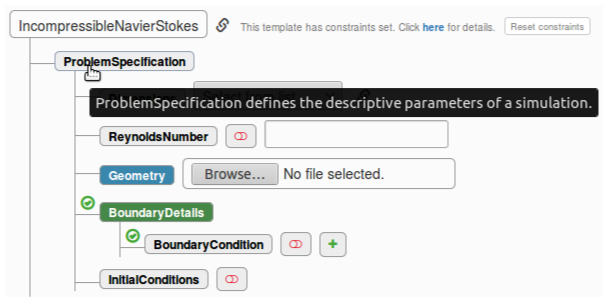
\includegraphics[width=.75\linewidth,  clip=true, trim = 0cm 0cm 0cm 0cm]{documentation}
 \captionof{figure}{Accessing Documentation Available for Nodes.}
 \label{fig:documentation}
\end{figure}

As previously remarked when designing the interface it is integral to keep related parameters within the same branch. However there are of course a number of parameters which have relationships across branches, these should be where possible linked through a set of constraints.

Names of nodes should be selected judiciously. Firstly they should have a name which represents their function, however in the documentation and input for Nektar++ they are often abreviated. Names should remain indicative as to which abreviated function, a node relates to, so that the user guides are not obselete within the context of TemPSS. Indeed this conflict is aided through the addition of comments to nodes that can elucidate the function of nodes, as pictured in figure \ref{fig:documentation}.

Ultimately the organisation of the branches, as listed in appendix \ref{app:tree_listing}, could take many forms. Thus the subsequent sections try to explain the rationale behind the combination of branches that has been chosen.

\subsection{Problem Specification}
When writing the abstract describing simulations of flow problems for a journal paper the authors will immediately answer four questions:
\begin{enumerate}
\item What is the domain of the simulation, is it 2D or 3D?
\item At which Reynolds number is this being simulated?
\item What boundary conditions are enforced?
\item Are there any initial conditions?
\end{enumerate}

The problem specification branch, see figure \ref{fig:problem_spec}, allows the immediate answering of these questions. Allowing the researcher to define fundamental simulation parameters, upload the geometry, specifiy boundary conditions, and initial conditions whether from file or expression.	

\newpage
\subsection{Numerical Specification}
Having now defined the simulation domain, users now would need to think how and what kind of problem they are solving. Therefore in the numerical specification branch a key node is \texttt{SimulationType}.

Three simulation types are available:
\begin{itemize}
\item Direct Numerical Simulation
\item Stability Analysis
\item Steady State Stability Analysis
\end{itemize}

These options are not real parameters specifiable within the code. Rather they are \textit{dummy} parameters which represent types of simulation that are possible to perform in Nektar++. Selection of a dummy parameter gives only the functions that are relevant to each kind of simulation. For example a DNS simulation gives the option to specificy the time integration method, driver type, but unlike in the stability analyses, no evolution operator. Furthermore the driver types are limited to only those which are used in DNS, standard and adaptive. Thereby shaping the options that are available to users, depending on what kind of analysis they wish to perform.

Additionally in the numerical specification the user defines the solver and equation types. Though they are again constrained in these choices depending on previous decisions, as detailed in section \ref{sec:constraints}.

\subsection{Additional Parameters}
Aside from the definition of the domain and selection of numerics there are a number of options which users may require. The additional parameters branch contains such options. For example the value of kinematic viscosity is used often in Nektar++, however it isn't a parameter which one would use to describe the simulation to a colleague. Therefore it requires inclusion but not in the problem specification branch, neither does it fit in the numerical specification branch. 

Additionally a number of analytical tools are listed here. Both filters and functions are commonly used tools to calculate the lift and drag across a body amongst others. However they are also optional and case dependent ergo they reside in this section.

\subsection{Advanced Parameters}
Advanced parameters branch contains options which improve stability or accuracy of the results. Most simulations could be run without them but certain situations would benefit from their use. One could imagine the situation where a user is possibly getting spurious oscillations within their domain, and thus are advised to switch dealiasing on. The options in this branch in this branch have some advanced requirements, which can improve simulations however a complete novice user would and should not need to use these options.

\subsection{Optimsation}
Correctly defining the optimisation parameters can lead to improved performance, however injudicious choices will hamper performance. Therefore optimisation parameters are kept in their own branch where experienced users of Nektar++ can create example settings for various cases.

\begin{figure}[!htb]
\centering
\begin{subfigure}{.5\textwidth}
  \centering
  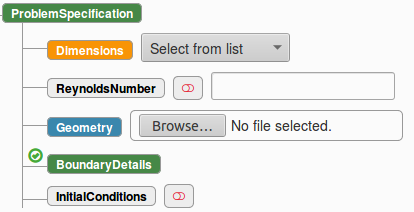
\includegraphics[width=1.\linewidth]{problem_spec}
  \caption{Problem Specification Branch.}
  \label{fig:problem_spec}
\end{subfigure}%
\begin{subfigure}{.5\textwidth}
  \centering
  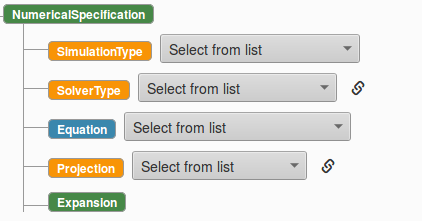
\includegraphics[width=1.\linewidth]{numerical_spec}
  \caption{Numerical Specification Branch.}
  \label{fig:numerical_spec}
\end{subfigure}
\caption{Visualisations of the Key Branches in the TemPSS Interface.}
\label{fig:branches}
\end{figure}

\section{Testing of the Interface}
In order to ensure that the user interface is intuitive a number of tests have been performed by users of Nektar++.

Three individuals were asked to use TemPSS to generate a test case of their choice. Below their recommendations and comments are listed with a brief explanation of the action taken. Further details of the case ran and other is given in appendix \ref{app:testing}.

\subsection{Recommendations and Actions}
\begin{multicols}{2}

\textbf{Recommendation:}
\begin{enumerate}
\item Speed up the from scratch profile instantiation time.
\item Reduce sensitivity of switches. Include additional filters.\\ 
\item Automate the boundary condition selection.\\
\end{enumerate}

\columnbreak

\textbf{Action Taken:}
\begin{enumerate}
\item Partial profile loading functionality is being developed.
\item Cannot do anything about button sensitivity. Additional filters, such as history points, have been added.
\item The field variables are now selected depending on dimensions and solver type.
\end{enumerate}

\end{multicols}

\chapter{Constraints}
\label{sec:constraints}
The TemPSS interface must encapsulate all of Nektar++'s parameter space whilst remaining intuitive to operate. Withal, when placed within the wider context of Nekkloud, it is highly undesirable if users are able to launch simulations which do not run - especially if cloud resources have been allocated and paid for! TemPSS must try to prevent or limit users from choosing options that are either incorrect, incompatible or irresponsible.

In order to map constraints between functions the work-flow, of instantiating a profile, should be determined. As users navigate through this work-flow options should come in and out of scope as appropriate.

\begin{figure}[htb!]
 \centering
 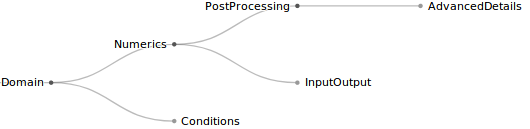
\includegraphics[width=.85\linewidth,  clip=true, trim = 0cm 0cm 0cm 0cm]{workflow}
 \captionof{figure}{Work Flow of Decisions Necessary to Create a Simulation.}
 \label{fig:descision_flow}
\end{figure}

\noindent
Constraints are then enforced through two different methods:
\begin{itemize}
\item Direct enforcement
\item Indirect enforcement
\end{itemize}

\subsection{Direct Constraints}
Direct constraint enforcement is the simplest to implement. Using an XML file parameters paths are defined and options listed. 
In figure \ref{fig:constraints_variables} possible options for solver type and projection are listed.

\begin{figure}[htb!]
 \centering
 \lstinputlisting{./data/constraints_variables.xml}
 \captionof{figure}{Example Constraint File Showing the Listing of Solver Types and Projections.}
 \label{fig:constraints_variables}
\end{figure}

In figure \ref{fig:constraints_mapping} the solver type and projection are directly linked. Specific variables have compatible target variables listed beneath each value. For the coupled linear Navier-Stokes solver only the continuous galerkin projection is available. Whereas, for the velocity correction scheme all three projection types are available. The constraint file prevents values being chosen if another option does not list an value as valid, as in figure \ref{fig:constraints_mapping}. Additionally a small guide, as in figures \ref{fig:constraint_info} and \ref{fig:constraint_info_2}, details the variables and values which are constrained.

\begin{figure}[htb!]
 \centering
 \lstinputlisting{./data/constraints_mapping.xml}
 \captionof{figure}{Example Constraint File Showing the Linking of Projection Types to Solvers.}
 \label{fig:constraints_mapping}
\end{figure}

\begin{figure}[!htb]
\centering
\begin{subfigure}{.5\textwidth}
  \centering
  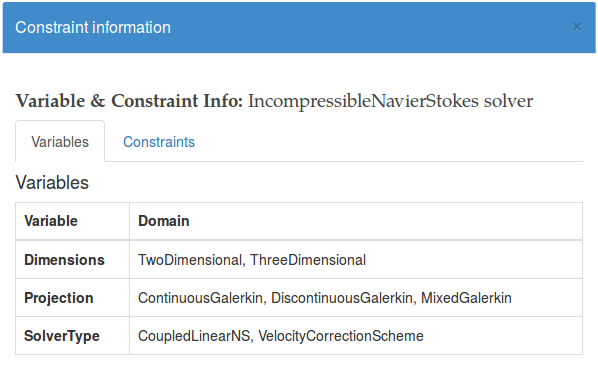
\includegraphics[width=.9\linewidth]{constraint_info}
  \caption{Constraint Info: Variables.}
  \label{fig:constraint_info}
\end{subfigure}%
\begin{subfigure}{.5\textwidth}
  \centering
  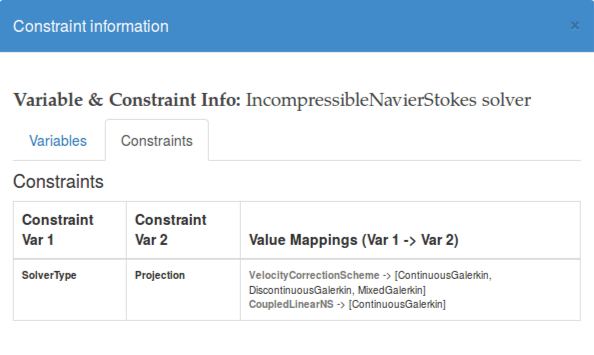
\includegraphics[width=.975\linewidth]{constraint_info_2}
  \caption{Constraint Info: Constraints.}
  \label{fig:constraint_info_2}
\end{subfigure}
\caption{Information Widget Available in TemPSS Showing a List of Constraints Enforced in the Parameter Space.}
\label{fig:constrain}
\end{figure}

\subsection{Indirect Constraints}
Indirect or implicit constraints are somewhat more subtle than the explicitly defined constraints. Through creation of various templates, for certain common functions, the tree can be altered depending upon which kind of simulation is being performed. This occurs for the dummy parameter of \texttt{simulationType}. Here the option \texttt{EvolutionOperator} does not appear if \texttt{DirectNumericalSimulation} is chosen. Whereas for both other simulation types it does.

\section{Mapping Constraints}
Prior to enforcing the constraints between parameters within the solver, the entire parameter space must be determined. Within this space only a subset of parameters have relationships. For the incompressible Navier-Stokes solver the linked parameters are listed below:
\begin{multicols}{3}
\begin{itemize}
\item Dimensions 
\item Equation Type
\item Field Details
\item Simulation Type
\item Time Integration Details
\item Evolution Operator
\item Solver Type
\item Boundary Conditions
\item Driver Type
\end{itemize}
\end{multicols}
Using documentation, examples, and testing the dependencies have been ascertained and constraints implemented. Furthermore to help easily understand these relationships have been mapped out visually, see appendix \ref{app:constraints}. The use of this graph is subsequently discussed in section \ref{sec:constraint_graph}.

\subsection{Dimensions, Solver Type, and Field}
When instantiating a simulation the user will need to understand what domain they are studying, and thus select the dimensions. Having chosen whether the domain is 2D or 3D, and if any of these are quasi-dimensions, the user has determined whether the velocity field contains $u, v$ and $w$. Corollary to this, selection of solver type determines if the solution of pressure $p$ field is required.

Knowing the dimensions, solver type and therefore the solution fields has consequences in the definition of boundary conditions and expansion. To prevent the incorrect field values being selected, the XML schema automatically selects the correct variables in the boundary conditions and for a simple expansion.

\begin{figure}[!htb]
\centering
\begin{subfigure}{.5\textwidth}
  \centering
  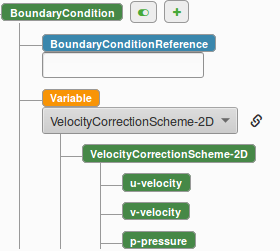
\includegraphics[width=.9\linewidth]{VCS_2D}
  \caption{Velocity Correction Scheme 2D.}
  \label{fig:vcs2d}
\end{subfigure}%
\begin{subfigure}{.5\textwidth}
  \centering
  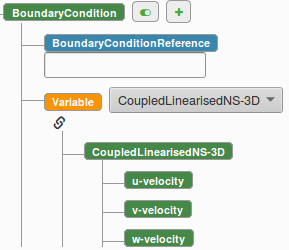
\includegraphics[width=.9\linewidth]{coupledLinear3D}
  \caption{Coupled Linear Navier-Stokes 3D.}
  \label{fig:coupledlinear3d}
\end{subfigure}
\caption{Comparison of the Automatically Selected Fields Used in Boundary Condition Definition.}
\label{fig:implicit_constraints}
\end{figure}

Figure \ref{fig:implicit_constraints} shows how the field choice restrictions manifest themselves in the template tree. In figure \ref{fig:vcs2d} the user started by selecting a two-dimensional domain and the the velocity correction scheme as solver type. Subsequently, when they tried to define the boundary conditions field variables $u, v$ and $p$ automatically appeared. Similarly, figure \ref{fig:coupledlinear3d} shows the variables that are presented when using the coupled linear Navier-Stokes solver for a 3D domain.

Here the impact of previous decisions is shown through the restriction of choices available. Important to note is that the directionality of decisions is reversable. Insomuch that the user may start to instantiate a profile anywhere in the tree and constraints will still be enforced identically.

\subsection{Geometry and Boundary Conditions}
In the previous section the user defined the dimensions, solver type and field. Having selected these parameters the boundary conditions should be defined and applied.

\begin{figure}[htb!]
 \centering
 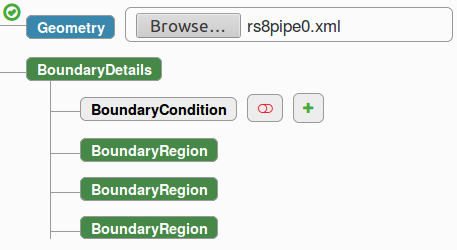
\includegraphics[width=.6\linewidth,  clip=true, trim = 0cm 0cm 0cm 0cm]{geometry_upload}
 \captionof{figure}{Boundary Regions Identified In Uploaded Geometry File.}
 \label{fig:geometry_upload}
\end{figure}

TemPSS allows the user to browse their filesystem to a Nektar++ compatible XML geometry file and upload it. Doing so both allows the geometry to be included in the final TemPSS generated output XML reducing the number of files needed to start a simulation. Additionally the geometry file is scanned for boundary composites. These composites are regions to which a bondition could be applied ubiquitously. Figure \ref{fig:geometry_upload} shows the identified boundary regions for a pipe geometry. These regions should then be linked to boundary conditions, via their boundary reference, as in figure \ref{fig:implicit_constraints}.

\subsection{Simulation Parameters}
Reduction in time spent generating the input XMLs is a key goal of TemPSS. Through use of \textit{dummy} parameters the number of options available to the user, at any one time, is limited. These parameters are not Nektar++ related but encapsulate three fundamental types of simulation possible to run using Nektar++'s incompressible flow solver.
\begin{itemize}
\item Direct Numerical Simulation
\item Stability Analysis
\item Steady State Stability Analysis
\end{itemize}

\begin{figure}[!htb]
\centering
\begin{subfigure}{.5\textwidth}
  \centering
  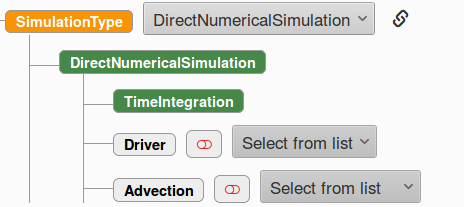
\includegraphics[width=1\linewidth]{dns}
  \caption{Direct Numerical Simulation.}
  \label{fig:dummy_dns}
\end{subfigure}%
\begin{subfigure}{.5\textwidth}
  \centering
  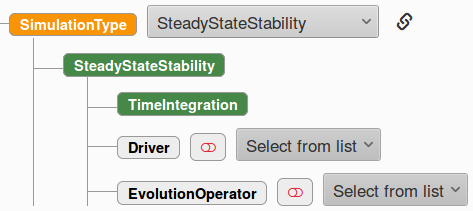
\includegraphics[width=1\linewidth]{steady_stability}
  \caption{Steady State Stability.}
  \label{fig:dummy_steady_state}
\end{subfigure}
\caption{Comparison of Dummy Parameter Selections.}
\label{fig:dummy_params}
\end{figure}

Shown in figure \ref{fig:dummy_params} the dummy parameters for the DNS and steady-state stability simulation types are shown. For the DNS the advection type appears whereas for the steady state stability it is replaced by the evolution operators. In this way the number of options available at any one time can be limited simplifying the interface for users.

\subsubsection{Direct Numerical Simulation}
\nomenclature{DNS}{Direct Numerical Simulation}
Direct numerical simulation is most commonly used simulation type in Nektar++'s incompressible solver. In order to run a DNS users must define time integration details. Driver and the advection types can also be specified, however the driver type is limited to the standard and adaptive configurations.

\subsubsection{Stability Analysis}
Hydrodynamic stability is a fundamental part of fluid dynamics. It allows the study of the development of turbulent states of motion from unstable flows. Nektar++ allows the study of  hydrodynamic stability of flows utilising a direct numerical simulation of the linearised Navier-Stokes equations using iterative methods for computing the solution of the associated eigenproblem.

\subsubsection{Steady State Stability Analysis}
\nomenclature{SFD}{Selective Frequency Damping}
Steady state stability analysis computes the steady state Naviers-Stokes equations in order to create a base flow for the purposes of a linear stability analyses. In order to obtain a base flow from potentially unstable flows selective frequency damping is used. The evolution operator is thus limited to SFD modes.

\subsection{Equation Type and Simulation Parameters}
Nektar++ solves the incompressible Navier-Stokes equations with a forcing term, defined as follows:
\begin{equation}
\frac{\partial \mathbf{u}}{\partial t} + \mathbf{u} \cdot \nabla \mathbf{u} = - \nabla p + \nu \nabla^{2} \mathbf{u} + \mathbf{f}, \qquad \nabla \cdot \mathbf{u} = 0
\label{eq:IncNS}
\end{equation}

\noindent
Further to this a number of additional formulations of the above equations are available:
\begin{itemize}
\item Steady Stokes
\item Steady Oseen
\item Steady Linearised Navier-Stokes
\item Unsteady Stokes
\item Unsteady Navier-Stokes
\end{itemize}

\subsubsection{Steady Stokes}
The incompressible Navier-Stokes equation is given in full in equation \ref{eq:IncNS}. However for the case $Re \ll 1$ the momentum component, $\frac{D \mathbf{u}}{D t}$, can be dropped from the full equation. Such a reduction is known as Stokes flow and represents the case of flows at extremely small length scales and velocities.

\begin{equation}
\nabla p - \nu \nabla^{2} \mathbf{u} = \mathbf{f}, \qquad \nabla \cdot \mathbf{u} = 0
\label{eq:SteadyStokes}
\end{equation}

As the Stokes equations are a linearised form of the full incompressible Navier-Stokes equations there is no time dependency other than that imposed by boundary conditions. Therefore the steady stokes requires only direct methods to find a solution.

\subsubsection{Steady Oseen}
The steady Oseen equations were derived by Oseen\cite{Oseen1910} as a development to the Stokes equations. The key difference between them is the inclusion of the convective acceleration.

\begin{equation}
\mathbf{u} \cdot \nabla \mathbf{u} + \nabla p - \nu \nabla^{2} \mathbf{u} = \mathbf{f}, \qquad \nabla \cdot \mathbf{u} = 0
\label{eq:SteadyOseen}
\end{equation}

\subsubsection{Steady Linearised Navier-Stokes}
The linearised Navier-Stokes equations are formed through the perturbation of the flow field. Considering the flow field as a steady base flow with the addition of minute perturbations,
\begin{equation}
\mathbf{u} = \mathbf{U} + \varepsilon\mathbf{u'}
\end{equation}
assuming that the $\varepsilon \ll 1$ the $\mathbf{u'} \cdot \mathbf{u'}$ terms can be neglected. This gives rise to the unsteady linearised Navier-Stokes equation:
\begin{equation}
\frac{\partial \mathbf{u'}}{\partial t} + \mathbf{U} \cdot \nabla \mathbf{u'} + \mathbf{u'} \cdot \nabla \mathbf{U} = - \nabla p + \nu  \nabla^{2} \mathbf{u'} + \mathbf{f}, \qquad \nabla\cdot\mathbf{u'} = 0
\label{eq:UnsteadyLinearisedNS}
\end{equation}
Performing the same operation to the steady Navier-Stokes gives the linearised Navier-Stokes:

\begin{equation}
\mathbf{u'} \cdot \nabla \mathbf{U} = - \nabla p + \nu  \nabla^{2} \mathbf{u'} + \mathbf{f}, \qquad \nabla\cdot\mathbf{u'} = 0
\label{eq:SteadyLinearisedNS}
\end{equation}

\subsubsection{Unsteady Stokes}
Similarly to the Oseen equations the unsteady Stokes equations seek to include accelerative terms, however in an unsteady equation. In this case the unsteady $\frac{\partial u}{\partial t}$ is included.

\begin{equation}
\frac{\partial \mathbf{u}}{\partial t} + \nabla p - \nu \nabla^{2} \mathbf{u} = \mathbf{f}, \qquad \nabla \cdot \mathbf{u} = 0
\label{eq:UnsteadyStokes}
\end{equation}

\subsubsection{Unsteady Navier-Stokes}
The final form, and most commonly used, of the equation that the incompressible Navier-Stokes solver can operate on is the full unsteady Navier-Stokes equations as in equation \ref{eq:IncNS}.
		
\subsubsection{Relationship with Solver Type}
Each equation has a direct relationship with the solver that is available to use. Ergo when a solver is chosen, within the TemPSS tree, the equation types become restricted. These relations are listed directly in the Nektar++ user documentation and again reproduced in table \ref{tab:equation_solver_relation}. Enforcement of these relationships is performed directly through use of the XML constraint file.

\begin{table}[htb!]
	\centering
    \begin{tabular}{ l || c | c }
    \hline
    Equation & Velocity Correction Scheme & Coupled Linearised Navier-Stokes\\
    \hline
    Steady Oseen &  & \checkmark \\
    Steady Stokes & \checkmark & \\
    Steady Linearised Navier-Stokes & & \checkmark \\
    Unsteady Stokes & \checkmark & \\
    Unsteady Navier-Stokes & \checkmark & \\
    \hline
    \end{tabular}
    \caption{Relationship Between Equation and Solver Types.}
    \label{tab:equation_solver_relation}
\end{table}

\subsubsection{Relationship with Simulation Type}
Along with the choice of solver the equation type is also restricted through the simulation type. Table \ref{tab:equation_simulation_relation} shows the direct relations. These relations are derived from the test and examples cases in Nektar++, but also from the user documentation.

When performing direct numerical simulations all velocity scales are being resolved. In order to capture all the scales the equations cannot be linearised or other therefore the only suitable equation type is that of the unsteady Navier-Stokes.

For the case of stability analysis the Navier-Stokes equations should be written in the perturbed form, thus the steady linearised form is available. However using the appropriate drivers and evolution operators allows the stability analysis to be performed using both the unsteady Stokes and full Navier-Stokes equations.

Steady-State Stability analyses implement the classical and adaptive SFD in order to determine a base flow for further stability analyses.  Typically these base flows are derived from fully turbulent simulations hence the unsteady Navier-Stokes is often used. However it also possible to utilise the Steady Oseen and Stokes equations to create a base flow.

\begin{table}[htb!]
	\centering
    \begin{tabular}{ l || c | c | c}
    \hline
    Equation & DNS & Stability & Steady-State\\
    \hline
    Steady Oseen & & & \checkmark \\
    Steady Stokes & & & \checkmark \\
    Steady Linearised Navier-Stokes & & \checkmark &\\
    Unsteady Stokes & & \checkmark & \\
    Unsteady Navier-Stokes & \checkmark & \checkmark & \checkmark\\
    \hline
    \end{tabular}
    \caption{Relationship Between Equation and Simulation Types.}
    \label{tab:equation_simulation_relation}
\end{table}

\subsection{Timing Details}
Timing details, whilst crucial for the output of a physical solution, are dependent directly upon the choice of equation type. However equations available differs for each simulation and solver type.

In effect the equations are split into two groups; those that require time integration, and those that are solved directly. Deducing which equations fall into either category however is not simple, and has been compeleted through testing.

\begin{table}[htb!]
	\centering
    \begin{tabular}{ l || c | c }
    \hline
    Equation Type & No Time Integration & Time Integration \\
    \hline
    Steady Oseen &  & \checkmark \\
    Steady Stokes & \checkmark & \\
    Steady Linearised Navier-Stokes & & \checkmark \\
    Unsteady Stokes & \checkmark & \\
    Unsteady Navier-Stokes & \checkmark & \\
    \hline
    \end{tabular}
    \caption{Relationship Between Equation and Solver Types.}
    \label{tab:equation_solver_relation}
\end{table}

Additionally solver types, coupled linear Navier-Stokes and velocity correction schemes, are explicitly linked to equation types in the Nektar++ documentation. Therefore an indirect restriction on timing details is placed from the simulation types.

\subsection{Driver Type}
Drivers manage the simulation at a high-level. Within the incompressible Navier-Stokes solver five separate drivers exist. Specifying no driver is equivocal to selecting the standard driver. Selecting a different driver effectively changes the simulation type that is being run. Ergo if a standard driver is chosen then DNS is being performed whereas selecting the steady state indicates that a steady stability analysis is to be run. A brief synopsis is given by table \ref{tab:driver_simulation_relation}.

\begin{table}[htb!]
	\centering
    \begin{tabular}{ l || c | c | c}
    \hline
    Driver Type & DNS & Stability & Steady-State\\
    \hline
    Standard & \checkmark &  \checkmark & \\
    Adaptive & \checkmark & &\\
    Arpack & & \checkmark & \\
    Modified Arnoldi & & \checkmark &\\
    Steady State & & & \checkmark \\
    \hline
    \end{tabular}
    \caption{Relationship Between Driver and Simulation Types.}
    \label{tab:driver_simulation_relation}
\end{table}

For DNS the available drivers are the standard and adaptive. Standard driver completes a number of tasks; prints a summary of conditions defined; sets up initial and boundary conditions; calls the solver type; and writes the outputs to a .fld. However if a user wishes to utilise adaptive polynomial ordering then they are to use the adaptive driver which is required when running quasi-dimension problems.

If a stability analysis is being run the drivers available, including standard, are the modified Arnoldi and Arpack. Modified Arnoldi driver computes a number of leading eigenvalues and eigen modes, thus making it suitable for stability analyses. Similarly the Arpack driver allows a solution of eigenmodes using a selection of other methods.

For steady state stability analysis the only option available is the steady state driver.

\subsection{Evolution Operators}
Evolution operators allow the study of the change in pertubations in stability analyses. Each operator slightly alters the Navier-Stokes equations and therefore they are exclusive to both forms of stability analysis.

\begin{table}[htb!]
	\centering
    \begin{tabular}{ l || c | c }
    \hline
    Evolution Operator & Stability & Steady-State\\
    \hline
    Adjoint & \checkmark & \\
    Direct & \checkmark & \\
    NonLinear & \checkmark &	 \\
    Skew Symmetric & \checkmark &\\
    Transient Growth & \checkmark &\\
    Classical SFD & &\checkmark \\
    Adaptive SFD & &\checkmark \\
    \hline
    \end{tabular}
    \caption{Relationship Between Driver and Simulation Types.}
    \label{tab:driver_simulation_relation}
\end{table}

For the adaptive SFD operator a number of additional parameters are required. Selecting this operator then opens a sub-tree from which these options can be defined, see figure \ref{fig:evop_adaptiveSFD}. This again highlights how the XML schema can be used to bring variables in and out of scope.

\begin{figure}[htb!]
 \centering
 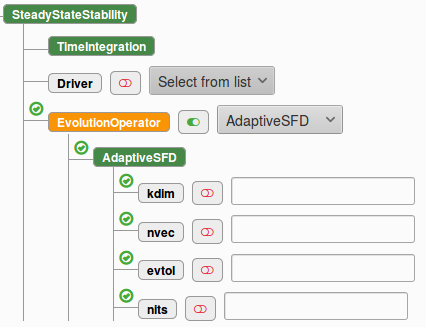
\includegraphics[width=.55\linewidth,  clip=true, trim = 0cm 0cm 0cm 0cm]{evop_adaptiveSFD}
 \captionof{figure}{Snippet of Tree Showing Sub-trees for Specification of AdaptiveSFD Evolution Operator.}
 \label{fig:evop_adaptiveSFD}
\end{figure}

\section{Constraints Graph}
\label{sec:constraint_graph}
Visual tools are often the most effective at simply conveying the relationship between nodes in a network. Therefore a chord diagram was created, detailing the relationship between the parameter available within the incompressible flow solver. 

However simply connecting parameters together does not imply any directionality to the decisions. Therefore an interactive visualisation has been created which show the relationship of parameter pairs, and also gives a directionality between these relations. An example image of the chord graph, and instructions in how to access it is given in appendix \ref{app:constraints}.

\begin{figure}[htb!]
 \centering
 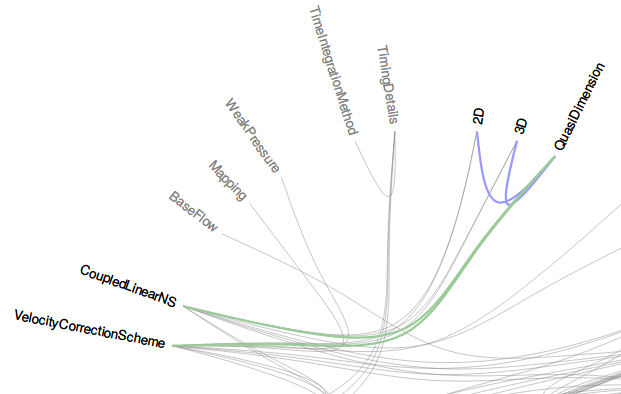
\includegraphics[width=.95\linewidth,  clip=true, trim = 0cm 0cm 0cm 0cm]{constraint_directionality}
 \captionof{figure}{Excerpt of Constraint Chord Diagram Showing Directionality of Choices.}
 \label{fig:constrain_directionality}
\end{figure}

Figure \ref{fig:constrain_directionality} shows a snippet of this interactive diagram. A user can select any parameter, with like parameters being grouped together. Once a parameter has been selected the links between related parameters are illuminated. Green shows that a link is dependent upon the selected parameters, speak this is a downwind selection. Whereas blue shows that the linked node is upstream of the selected parameter.

In the figure \ref{fig:constrain_directionality} the user has selected quasi dimensions. The blue links show that in order to select this the user should have chosen either 2D or 3D as the dimension field. The green shows that now the user can choose from either the coupled linear Navier-Stokes solver or velocity correction scheme. Moving then to the next option a user can see which other parameters become available and slowly navigate their way through the key decisions.

This tool is not only helpful in encapsulating these relationships clearly, but through definition of a simple \texttt{.json} file new relationships can be rapidly visualised.
%----------------------------------------------------------------------------------------
%	TESTING AND RESULTS
%----------------------------------------------------------------------------------------
\newpage
\chapter{Testing and Results}
TemPSS must be relied upon to accurately and consistently create functioning input files for Nektar++, which also prevent logical inconsistencies from being defined. To test that TemPSS is correctly generating XMLs, a number of test cases have been developed. These cases represent between them a wide variety of functionality of the incompressible Navier-Stokes solver.

\begin{itemize}
\item Flow past a NACA aerofoil
\item Simulation of T106a turbine blade using quasi-dimension
\item Fully-developed turbulent pipe flow
\end{itemize}

Developing the input files using TemPSS the results are then compared against the original simulations to ensure they produce identical results.

\section{NACA Aerofoil}
Simulation of the flow past a NACA aerofoil, at Reynolds number $135,000$, has been performed. This case tests a number of key functions in the incompressible Navier-Stokes solver. Moreover many of the potential Nekkloud users would wish to simulate flows past aerofoils and other aerodynamic components, thus demonstrating this capability is key to increasing user numbers.

\begin{table}[htb!]
	\centering
    \begin{tabular}{ c || c }
    \hline
    Boundary & Type \\
    \hline
    1 & Inlet \\
    2 & Periodic with 6\\
    3 & Periodic with 5\\
    4 & Outlet\\
    5 & Periodic with 3\\
    6 & Periodic with 2\\
    7 & Wall\\
    \hline
    \end{tabular}
    \caption{Boundary Conditions of the NACA Aerofoil Simulation.}
    \label{tab:naca_boundaries}
\end{table}

Domain of the simulated NACA aerofoil is shown in figure \ref{fig:naca_domain}, with the boundaries labelled described in table \ref{tab:naca_boundaries}. To ensure that the simulations are being defined correctly two simulations have been run. The first the original input file defined manually, followed by the same simulation generated through TemPSS. Using the aerodynamic forces filter the lift and drag acting on the body has been calculated at a number of time intervals.

\begin{figure}[htb!]
 \centering
 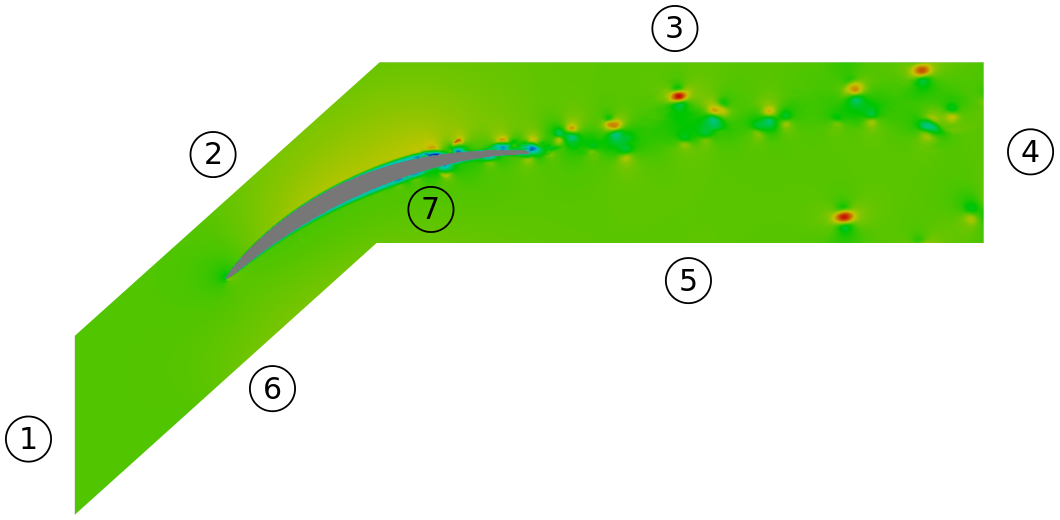
\includegraphics[width=.75\linewidth,  clip=true, trim = 0cm 0cm 0cm 0cm]{naca_domain}
 \captionof{figure}{Domain of the NACA Aerofoil.}
 \label{fig:naca_domain}
\end{figure}

Running for a total of 5000 time intervals the aerodynamic forces were measured every 1000 iterations. Results for both the original input file and that generated through TemPSS are list in table \ref{tab:aero_comparison}. Data from this table is subsequently visualised in figure \ref{fig:drag_lift_comparison} in which it can be clearly seen that both the drag forces for the original and TemPSS generated inputs are identical and thus for such cases TemPSS is working as expected.

\begin{figure}[htb!]
 \centering
 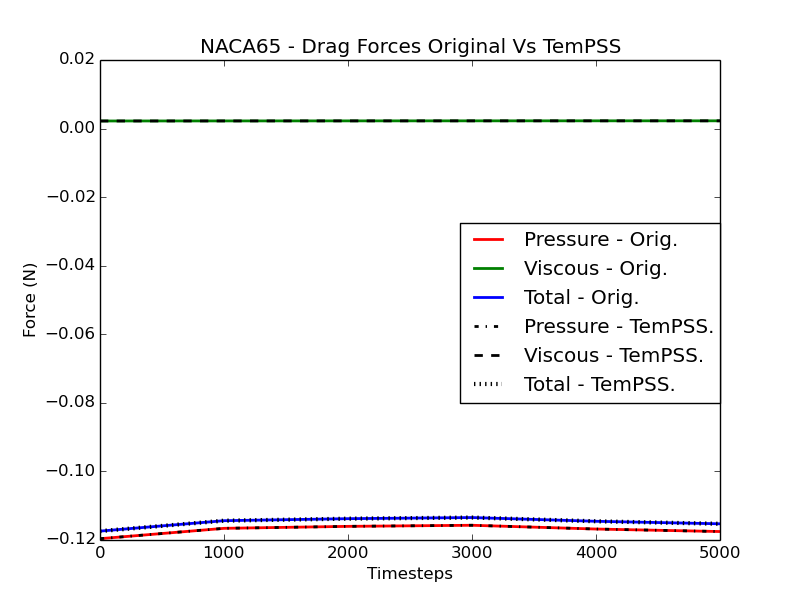
\includegraphics[width=.75\linewidth,  clip=true, trim = 0cm 0cm 0cm 0cm]{drag}
 \captionof{figure}{Comparison of Drag for Original and TemPSS Generated Input Files of NACA65.}
 \label{fig:drag_lift_comparison}
\end{figure}

\newpage
\section{T106a Quasi-3D Turbine Blade}
The case T106a simulates a turbine blade, pictured in figure \ref{fig:t106a_domain}, at Reynolds number $50,000$ and an angle of attack of $37.7^{\circ}$. Unique to this simulation is that a Fourier expansion is used to simulate in the homogeneous component.

\begin{figure}[htb!]
 \centering
 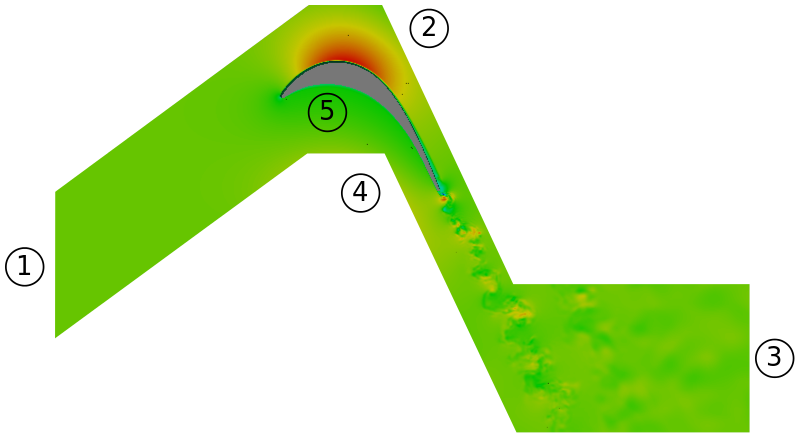
\includegraphics[width=.75\linewidth,  clip=true, trim = 0cm 0cm 0cm 0cm]{t106a_domain}
 \captionof{figure}{Domain of the T106a Turbine Blade.}
 \label{fig:t106a_domain}
\end{figure}

As with the simulation of the NACA65 profile above, TemPSS has been verified through the comparison of the drag and lift forces. Running for 20 timesteps only, and writing every 10, the drag force is shown in figure \ref{fig:drag_lift_t106a}. Additionally appendix \ref{app:drag_lift_t106a}  details the exact figures for both lift and drag from the original and TemPSS generated inputs. Again the drag and lift forces match identically so it can be infered that TemPSS is correctly generating the input XMLs.

\begin{figure}[htb!]
 \centering
 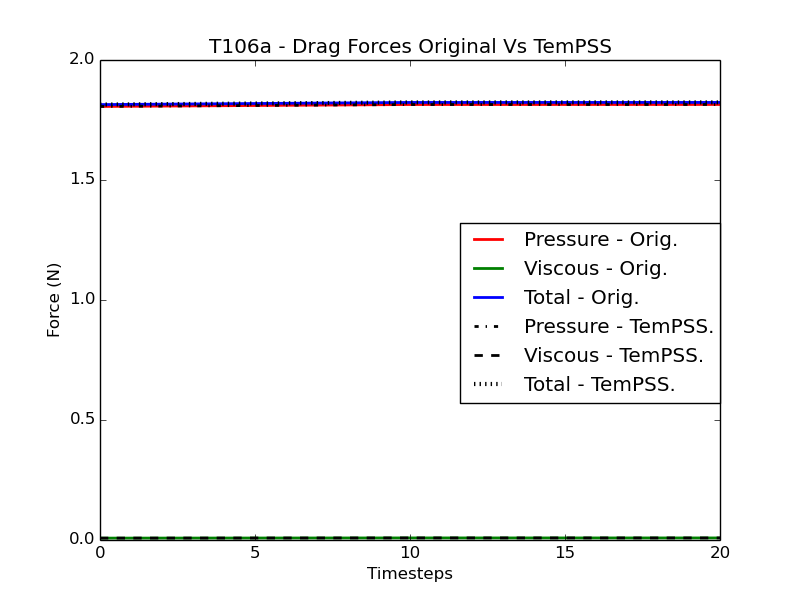
\includegraphics[width=.75\linewidth,  clip=true, trim = 0cm 0cm 0cm 0cm]{drag_t106a}
 \captionof{figure}{Comparison of Drag for Original and TemPSS Generated Input Files of T106a.}
 \label{fig:drag_lift_t106a}
\end{figure}

\begin{table}[htb!]
	\centering
    \begin{tabular}{ c || c }
    \hline
    Boundary & Type \\
    \hline
    1 & Inlet \\
    2 & Periodic with 4\\
    3 & Outlet\\
    4 & Periodic with 2\\
    5 & Wall\\
    \hline
    \end{tabular}
    \caption{Boundary Conditions of the T106a Turbine Blade Simulation.}
    \label{tab:t106a_boundaries}
\end{table}


\section{Turbulent Pipe Flow}
A fully-developed turbulent pipe flow, with a periodic boundary condition, has also been simulated. Pipe flow is one of the canonical flow cases and offers insight into many aspects of fundamental fluid mechanics, such as turbulence transition. This simulation tests the ability of TemPSS to start a classical DNS simulation with a fully turbulent restart file as the initial conditions.

\begin{figure}[htb!]
 \centering
 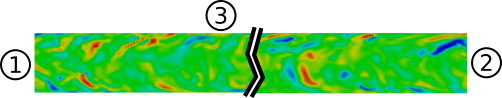
\includegraphics[width=.95\linewidth,  clip=true, trim = 0cm 0cm 0cm 0cm]{pipe_domain_real}
 \captionof{figure}{Domain of Turbulent Pipe.}
 \label{fig:pipe_domain}
\end{figure}

Checking that both input files are running an identical simulation the modal energy with time has been measured for each timestep. Shown in figure \ref{fig:pipe_modal} it is seen that both the original and TemPSS input have the same modal energies for the entire 1400+ timesteps of the simulation. The same procedure was performed for the simulation enstrophy and kinetic energies, giving an identical result.

\begin{table}[htb!]
	\centering
    \begin{tabular}{ c || c }
    \hline
    Boundary & Type \\
    \hline
    1 & Periodic with 2 \\
    2 & Periodic with 1\\
    3 & Wall \\
    \hline
    \end{tabular}
    \caption{Boundary Conditions of Pipe Simulation	.}
    \label{tab:pipe_boundaries}
\end{table}

\begin{figure}[htb!]
 \centering
 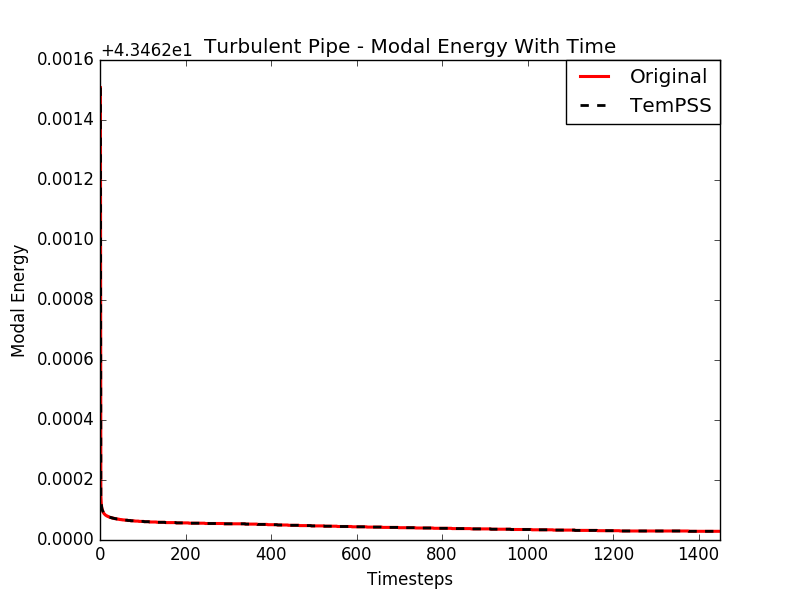
\includegraphics[width=.95\linewidth,  clip=true, trim = 0cm 0cm 0cm 0cm]{pipe_modal}
 \captionof{figure}{Modal Energy of Turbulent Pipe.}
 \label{fig:pipe_modal}
\end{figure}

%----------------------------------------------------------------------------------------
%	CONSTRAINTS AND FUTURE WORK
%----------------------------------------------------------------------------------------
\chapter{Conclusion and Further Work}
\section{Conclusion}
This report details the development and validation of a web-based graphical user interface named TemPSS. TemPSS generates input files for the incompressible flow solver in Nektar++. In aim of this the the incompressible Navier-Stokes solver parameter space has been encapsulated, mapped, and organised for intuitive operation of the graphical user interface. Included within this is the testing of the interface by a number of Nektar++ users. Additionally the relationships of between functions have been determined, mapped and visualised interactively, see appendix \ref{app:constraints}.

With respect to the original goals of the project, as defined in section \ref{chap:proj_spec}, the project can be deemed a success. However there is scope for further work and a number of recommendations for which are now presented.

\section{Further Work and Recommendations}
The principal objective of Nekkloud is the expansion of the user base for Nektar++. To fulfil this goal Nekkloud; simplifies the user interface of the code; reduces the expertise required by individuals to produce an actionable result; and gives direct access to HPC facilities. Within this there are a number of suggestions which would aid all three of these requirements:

\begin{enumerate}
\item Improve and consolidate the user eco-system within Nekkloud/Nektar++
\item Continue to add templates to TemPSS
\item Add the ability to load separate sections of profiles
\end{enumerate}

\subsection{Development of Nekkloud/Nektar++ Eco-System}
For users of Nektar++ outside of Imperial, or other supporting institutions, using the solvers requires following the documentation and tutorials available on the Nektar++ webpages. Whilst these resources are sophisticated and cater to a wide variety cases, there are inevitably a number of situations which require greater elucidation and/or support. In order to deal with these issues the users are given access to the core Nektar++ development team through a mailing list.

The Nekkloud platform has the potential to improve the quality of the support greatly. Immediately Nekkloud gives users the ability to utilise the code without the need to install locally, as they will utilise the cloud instances of Nektar++. However the most powerful way to improve the eco-system would be the inclusion of a forum in lieu of a mailing list. This is as:
\begin{itemize}
\item The mailing list has poor search facilities, and search functions in a forum would allows users to see if the same problem has previously been covered.
\item Queries posted to the mailing list are typically only answered by core Nektar++ developers. Using a forum allows for expertise generated within the user base to be leveraged in addition to the of the developers
\item As part of the separation of expertise rationale public profiles are available in TemPSS. Users may need a description of puplic profiles and a place to discuss them
\end{itemize}

Creation of a user community would also distinguish Nektar++ from \textit{competitor} codes. Many widely used codes do not have an online forum, however those that do have significantly higher user numbers.

\subsection{Creation of Additional Templates}
Within the scope of this project the only template developed was that of the incompressible Navier-Stokes solver. Though this is the most commonly used solver, addition of the compressible flow solver is an extremely important functionality for Nekkloud.

Though in effect the difference between the incompressible and compresible solvers is very little, as functions such as filters, optimisation, and so on are identical. There are however a number of differences in the equations used and the field which must be solver. Adding the compressible solver, and others, would need experienced use of the XML structure as to maximise the amount of code common to both solvers.

\subsection{Partial Profiles}
Part of the overall objective of this project is to separate the expertise required to run Nektar++. Though the ability to load pre-filled profiles edit and save the new versions is currently possible. It could be imagined that a user may wish to start a simulation from scratch knowing only the key parameters, i.e. those in the problem specification branch. Subsequently they could look through the available public profiles, select a branch from one and load it into their tree, perhaps then them may wish to repeat this. This functionality would greatly increase the speed at which simulations could be defined.

%---------------------------------------------------------------------------------------
%	BIBLIOGRAPHY
%---------------------------------------------------------------------------------------
\newpage
\bibliographystyle{unsrt}	% in order of appearance
%\bibliographystyle{acm}	% (uses file "plain.bst")
%\bibliographystyle{abbrv}	% (uses file "plain.bst")
%\bibliographystyle{siam}	% (uses file "plain.bst")
%\bibliographystyle{apalike}
\bibliography{/home/fmg215/Documents/latex/myrefs}		% expects file "myrefs.bib"}

%----------------------------------------------------------------------------------------
% APPENDIX
%----------------------------------------------------------------------------------------
\newpage
\appendix
\chapter{TemPSS Tree Listing}
\label{app:tree_listing}
\vspace*{-1cm}
These diagrams can be found at \url{https://github.com/maxrobot/chord_diag}. Instructions are listed in \url{README.md}.

\begin{figure}[htb!]
 \centering
 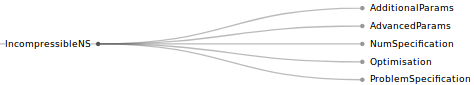
\includegraphics[width=.8\linewidth,  clip=true, trim = .1cm 0cm 0cm 0cm]{overview}
 \captionof{figure}{Diagrammatical Overview of Incompressible Navier-Stokes TemPSS Tree.}
 \label{fig:overview}
\end{figure}

\begin{figure}[htb!]
 \centering
 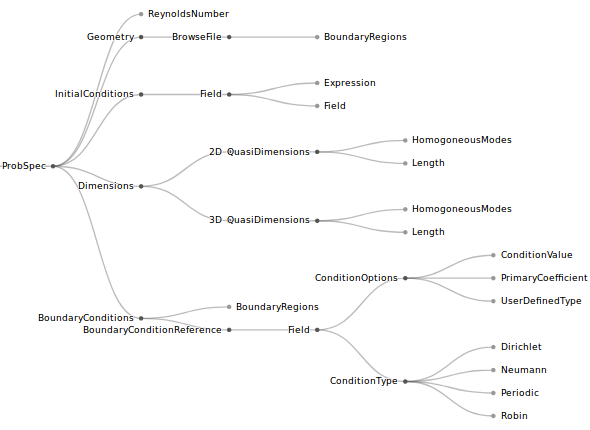
\includegraphics[width=1\linewidth,  clip=true, trim = 0cm 0cm 0cm 0cm]{problemSpecification}
 \captionof{figure}{Problem Specification Branch for Incompressible Navier-Stokes TemPSS Tree.}
 \label{fig:problemSpecification}
\end{figure}

\begin{figure}[htb!]
 \centering
 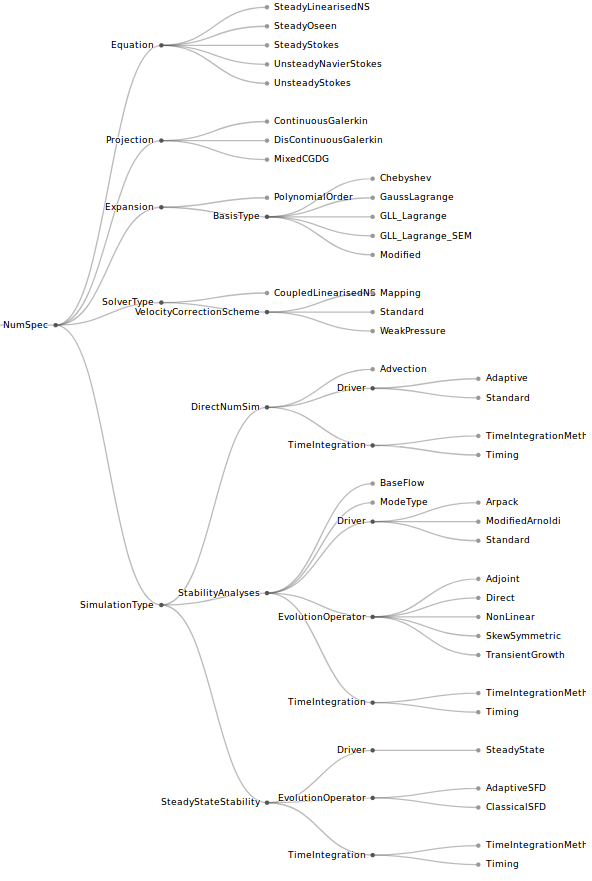
\includegraphics[width=1\linewidth,  clip=true, trim = .1cm 0cm 0cm 0cm]{numericalSpecification}
 \captionof{figure}{Numerical Specification Branch for Incompressible Navier-Stokes TemPSS Tree.}
 \label{fig:numericalSpecification}
\end{figure}

\begin{figure}[tb!]
 \centering
 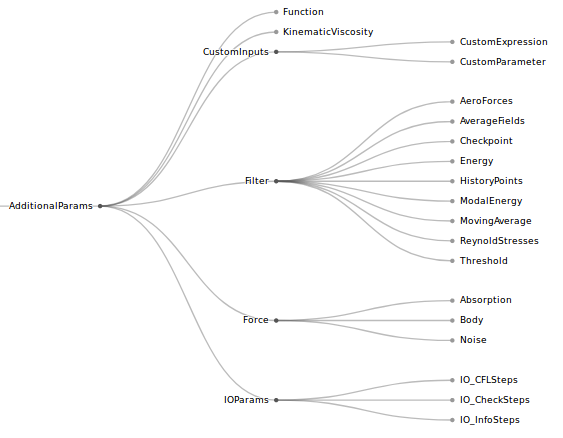
\includegraphics[width=1\linewidth,  clip=true, trim = .2cm 0cm 0cm 0cm]{AdditionalParameters}
 \captionof{figure}{Additional Parameters Branch for Incompressible Navier-Stokes TemPSS Tree.}
 \label{fig:problemSpecification}
\end{figure}

\begin{figure}[tb!]
 \centering
 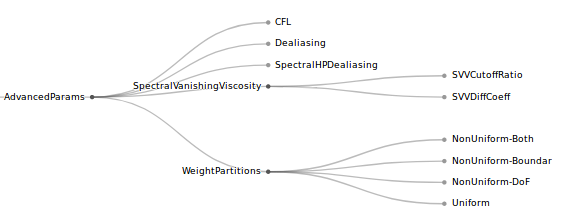
\includegraphics[width=1\linewidth,  clip=true, trim = .1cm 0cm 0cm 0cm]{AdvancedParameters}
 \captionof{figure}{Advanced Parameters Branch for Incompressible Navier-Stokes TemPSS Tree.}
 \label{fig:problemSpecification}
\end{figure}

\begin{figure}[tb!]
 \centering
 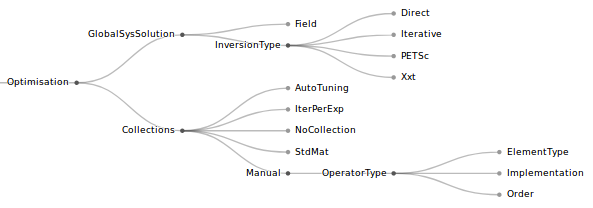
\includegraphics[width=1\linewidth,  clip=true, trim = .2cm 0cm 0cm 0cm]{optimisationb}
 \captionof{figure}{Optimisation Branch for Incompressible Navier-Stokes TemPSS Tree.}
 \label{fig:problemSpecification}
\end{figure}

\chapter{Interactive Constraint Visualiser}
\label{app:constraints}

\begin{figure}[htb!]
 \centering
 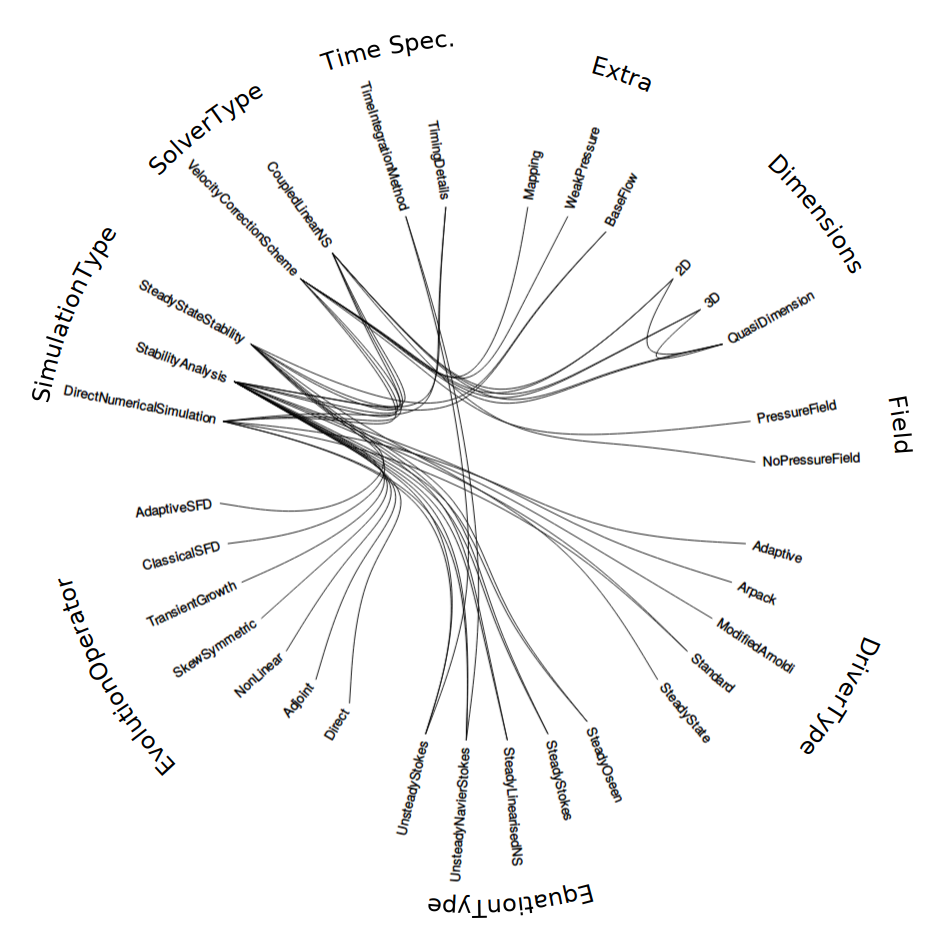
\includegraphics[width=.9\linewidth,  clip=true, trim = 0cm 0cm 0cm 0cm]{constraint_mapping}
 \captionof{figure}{Mapping of constraints between function for Nektar++ Incompressible Navier-Stokes Solver.}
 \label{fig:constraint_mapping}
\end{figure}

Figure \ref{fig:constraint_mapping} shows a still image of an interactive the map of relationships between functions available in Nektar++. Using an interactive map allowed the easy visualisation, and editing, of relationships between functions with directionality of dependence. Hovering over a function, with a mouse cursor, a green line is illuminated to the functions which are dependent on the function being chosen. Similarly a blue line shows backwards which functions are required to use a certain functionality.

This diagram can be found at \url{https://github.com/maxrobot/chord_diag}. Instructions are listed in \url{README.md}.

\chapter{NACA65 - Drag and Lift Force Measurement Comparison}
\label{app:drag_lift_comparison}
\begin{table}[htp]
    \centering
    \resizebox{\textwidth}{!}{
    \begin{tabular}{ c || c c c | c c c }
    \hline
	Timestep & Pressure x-axis & Viscous x-axis & Total x-axis & Pressure y-axis & Viscous y-axis & Total y-axis\\
    \hline
    0 & -0.11962121 & 0.002211952 & -0.11740926 & 0.23502283 & 0.0014489827 & 0.23647181\\
    1000 & -0.11659737 & 0.0022292138 & -0.11436815 & 0.23281936 & 0.0014352338 &  0.2342546\\
    2000 & -0.11602215 &  0.002242833 & -0.11377932 & 0.23268846 & 0.0014328509 & 0.23412131\\
    3000 & -0.11570363 & 0.0022527072 & -0.11345093 & 0.23299908 & 0.0014310583 & 0.23443014\\
    4000 & -0.11679946 & 0.0022576795 & -0.11454179 & 0.23428351 & 0.0014288948 &  0.2357124\\
    5000 & -0.11753313 & 0.0022588983 & -0.11527424 & 0.23468889 & 0.0014266195 & 0.23611551\\
    \hline
    \end{tabular}}
    \caption{Aeroforces NACA65 Original Input}
      \centering
     \resizebox{\textwidth}{!}{
    \begin{tabular}{ c || c c c | c c c }
    \hline
    Timestep & Pressure x-axis & Viscous x-axis & Total x-axis & Pressure y-axis & Viscous y-axis & Total y-axis\\
    \hline
    0 & -0.11962121 & 0.002211952 & -0.11740926 & 0.23502283 & 0.0014489827 & 0.23647181\\
    1000 & -0.11659737 & 0.0022292138 & -0.11436815 & 0.23281936 & 0.0014352338 &  0.2342546\\
    2000 & -0.11602215 &  0.002242833 & -0.11377932 & 0.23268846 & 0.0014328509 & 0.23412131\\
    3000 & -0.11570363 & 0.0022527072 & -0.11345093 & 0.23299908 & 0.0014310583 & 0.23443014\\
    4000 & -0.11679946 & 0.0022576795 & -0.11454179 & 0.23428351 & 0.0014288948 &  0.2357124\\
    5000 & -0.11753313 & 0.0022588983 & -0.11527424 & 0.23468889 & 0.0014266195 & 0.23611551\\
    \hline
    \end{tabular}}
	\caption{Aeroforces NACA65 TemPSS Generated Input}    	
    \label{tab:aero_comparison}
\end{table}

\chapter{T106a - Drag and Lift Force Measurement Comparison}
\label{app:drag_lift_t106a}
\begin{table}[htp]
    \centering
    \resizebox{\textwidth}{!}{
    \begin{tabular}{ c || c c c | c c c }
    \hline
	Timestep & Pressure x-axis & Viscous x-axis & Total x-axis & Pressure y-axis & Viscous y-axis & Total y-axis\\
    \hline
    0 & 1.8063751 & 0.0078590878 & 1.8142342 & 0.69212451 & -0.0080855233 & 0.68403899\\
	10 & 1.8144775 & 0.0086553326 & 1.8231328 & 0.69820648 & -0.0094729673 & 0.68873351\\
	20 & 1.8146635 & 0.0085670641 & 1.8232306 & 0.69832116 & -0.0093212748 & 0.68899988\\
    \hline
    \end{tabular}}
    \caption{Aeroforces T106a Original Input}
      \centering
     \resizebox{\textwidth}{!}{
    \begin{tabular}{ c || c c c | c c c }
    \hline
    Timestep & Pressure x-axis & Viscous x-axis & Total x-axis & Pressure y-axis & Viscous y-axis & Total y-axis\\
    \hline
    0 & 1.8063751 & 0.0078590878 & 1.8142342 & 0.69212451 & -0.0080855233 & 0.68403899\\
	10 & 1.8144775 & 0.0086553326 & 1.8231328 & 0.69820648 & -0.0094729673 & 0.68873351\\
	20 & 1.8146635 & 0.0085670641 & 1.8232306 & 0.69832116 & -0.0093212748 & 0.68899988\\
    \hline
    \end{tabular}}
	\caption{Aeroforces T106a TemPSS Generated Input}    	
    \label{tab:aero_comparison_t106a}
\end{table}

\chapter{Test TemPSS User Remarks}
\label{app:testing}

\section{User 1}
\textbf{Question 1:} What problem are you tring to solver?\\
I am always using the incompressible NS solver for problems of turbomachinery interest. I focus on both compressor and turbine blades, and for now I always use the 2.5D formulation with the Fourier expansion in the homogeneous direction. I always have some filters turned on, such as average fields, Reynolds stresses, history points and aerodynamic forces.\\
\textbf{Question 2:} Were you able to utilise TemPSS unaided?\\
I think with your explanation going through it the first time I was able to use it unaided, and it would actually be of help in case I had to create a case from scratch. In fact, I have never had to do so, always having a previous case from which to keep the structure of the session file.\\
\textbf{Question 3:} Do you have any recommendations?\\
The only recommendations would be aimed at speeding up the creation process the first time, but I do think it will be hard to figure out a way to do so - I'd say it's a pretty good tool already!

\section{User 2}
\textbf{Question 1:} What problem are you tring to solver?\\
I am studying the vortex interactions in the wake of a low incidence delta wing. Some PIV experiment was made a few years ago in Cambridge, and I am using the provided data to define my inlet boundary condition (velocity components in the plane straight after the wing). this boundary condition also defines my initial condition for convergence speed purpose. My domain of study is a box of size $1m*1m*1.18m$, meshed with 220+k tetrahedrons. My git branch is feature IncNS Sensor. The essential features used (apart from the common numerical definitions) are SpectralhpDealiasing, SpectralVanishingViscosity set to 'DGKernel' (feature not officially released) as well as GlobalSysSoln refinements. I am also using the History Points feature to study the velocity components in the vortex cores. I mostly run fifth and seventh order simulations (Nummodes = 6 and 8).\\
\textbf{Question 2:} Were you able to utilise TemPSS unaided?\\
I was able to use the software unaided.\\
\textbf{Question 3:} Do you have any recommendations?\\
Ensure that you do not have to click too specifically on the buttons. Also include the filter history points please.

\section{User 3}
\textbf{Question 1:} What problem are you tring to solver?\\
My cases are that of stability past a cylinder using eigenvalue analysis.\\
\textbf{Question 2:} Were you able to utilise TemPSS unaided?\\
Using the interface to define the numerical methods was fine but I had some problem defining the boundary fields.\\
\textbf{Question 3:} Do you have any recommendations?\\
It would be useful if there was a way to make the boundary condition definition more rapid, because it is very slow to fill them out one by one. But actually it is better than using the terminal for the first time.

%----------------------------------------------------------------------------------------
% END DOCUMENT
%----------------------------------------------------------------------------------------
\end{document}